\subsection{27 августа. Пер. Перемётный (1А)}
\textit{Метеоусловия: утром, днём, вечером ясно, тепло.}

\begin{figure}[h!]
	\centering
	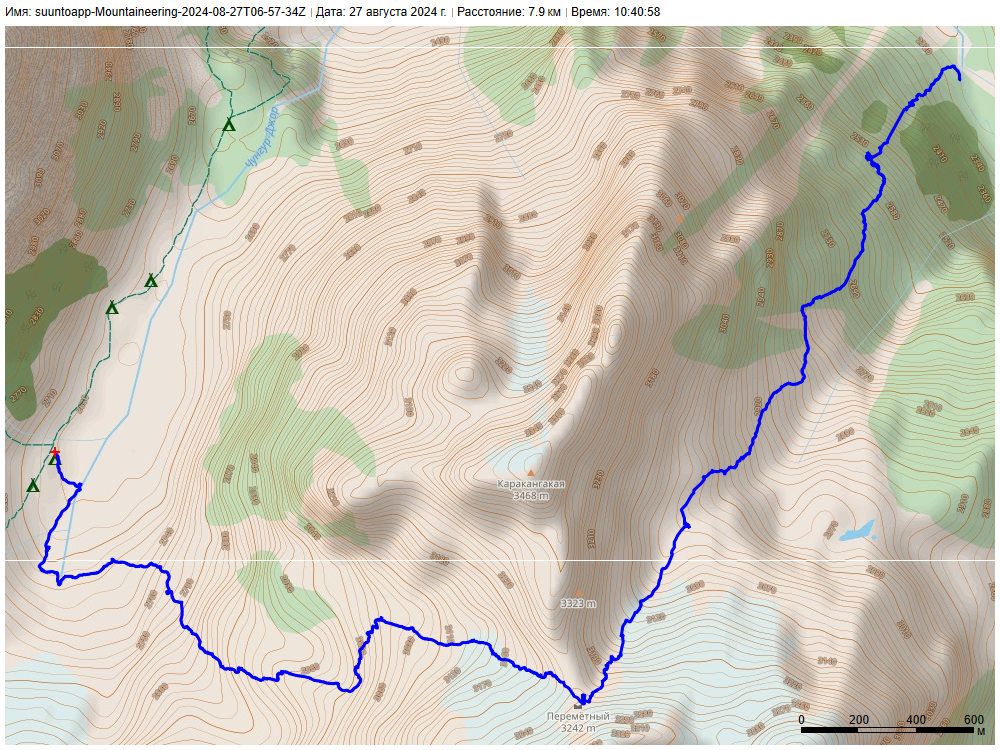
\includegraphics[angle=0, width=0.7\linewidth]{../pics/mini_maps/27}
	\label{fig:mini_27}
\end{figure}

Утром проснулись в 7:00. Погода прекрасная: небо ясное, долину постепенно заливает солнцем. Долго стирались, чинились и сушились, руковод курил какао и размышлял... Перемётный было решено брать!
В 10:00 выдвинулись в сторону перевала.

\begin{figure}[h!]
	\centering
	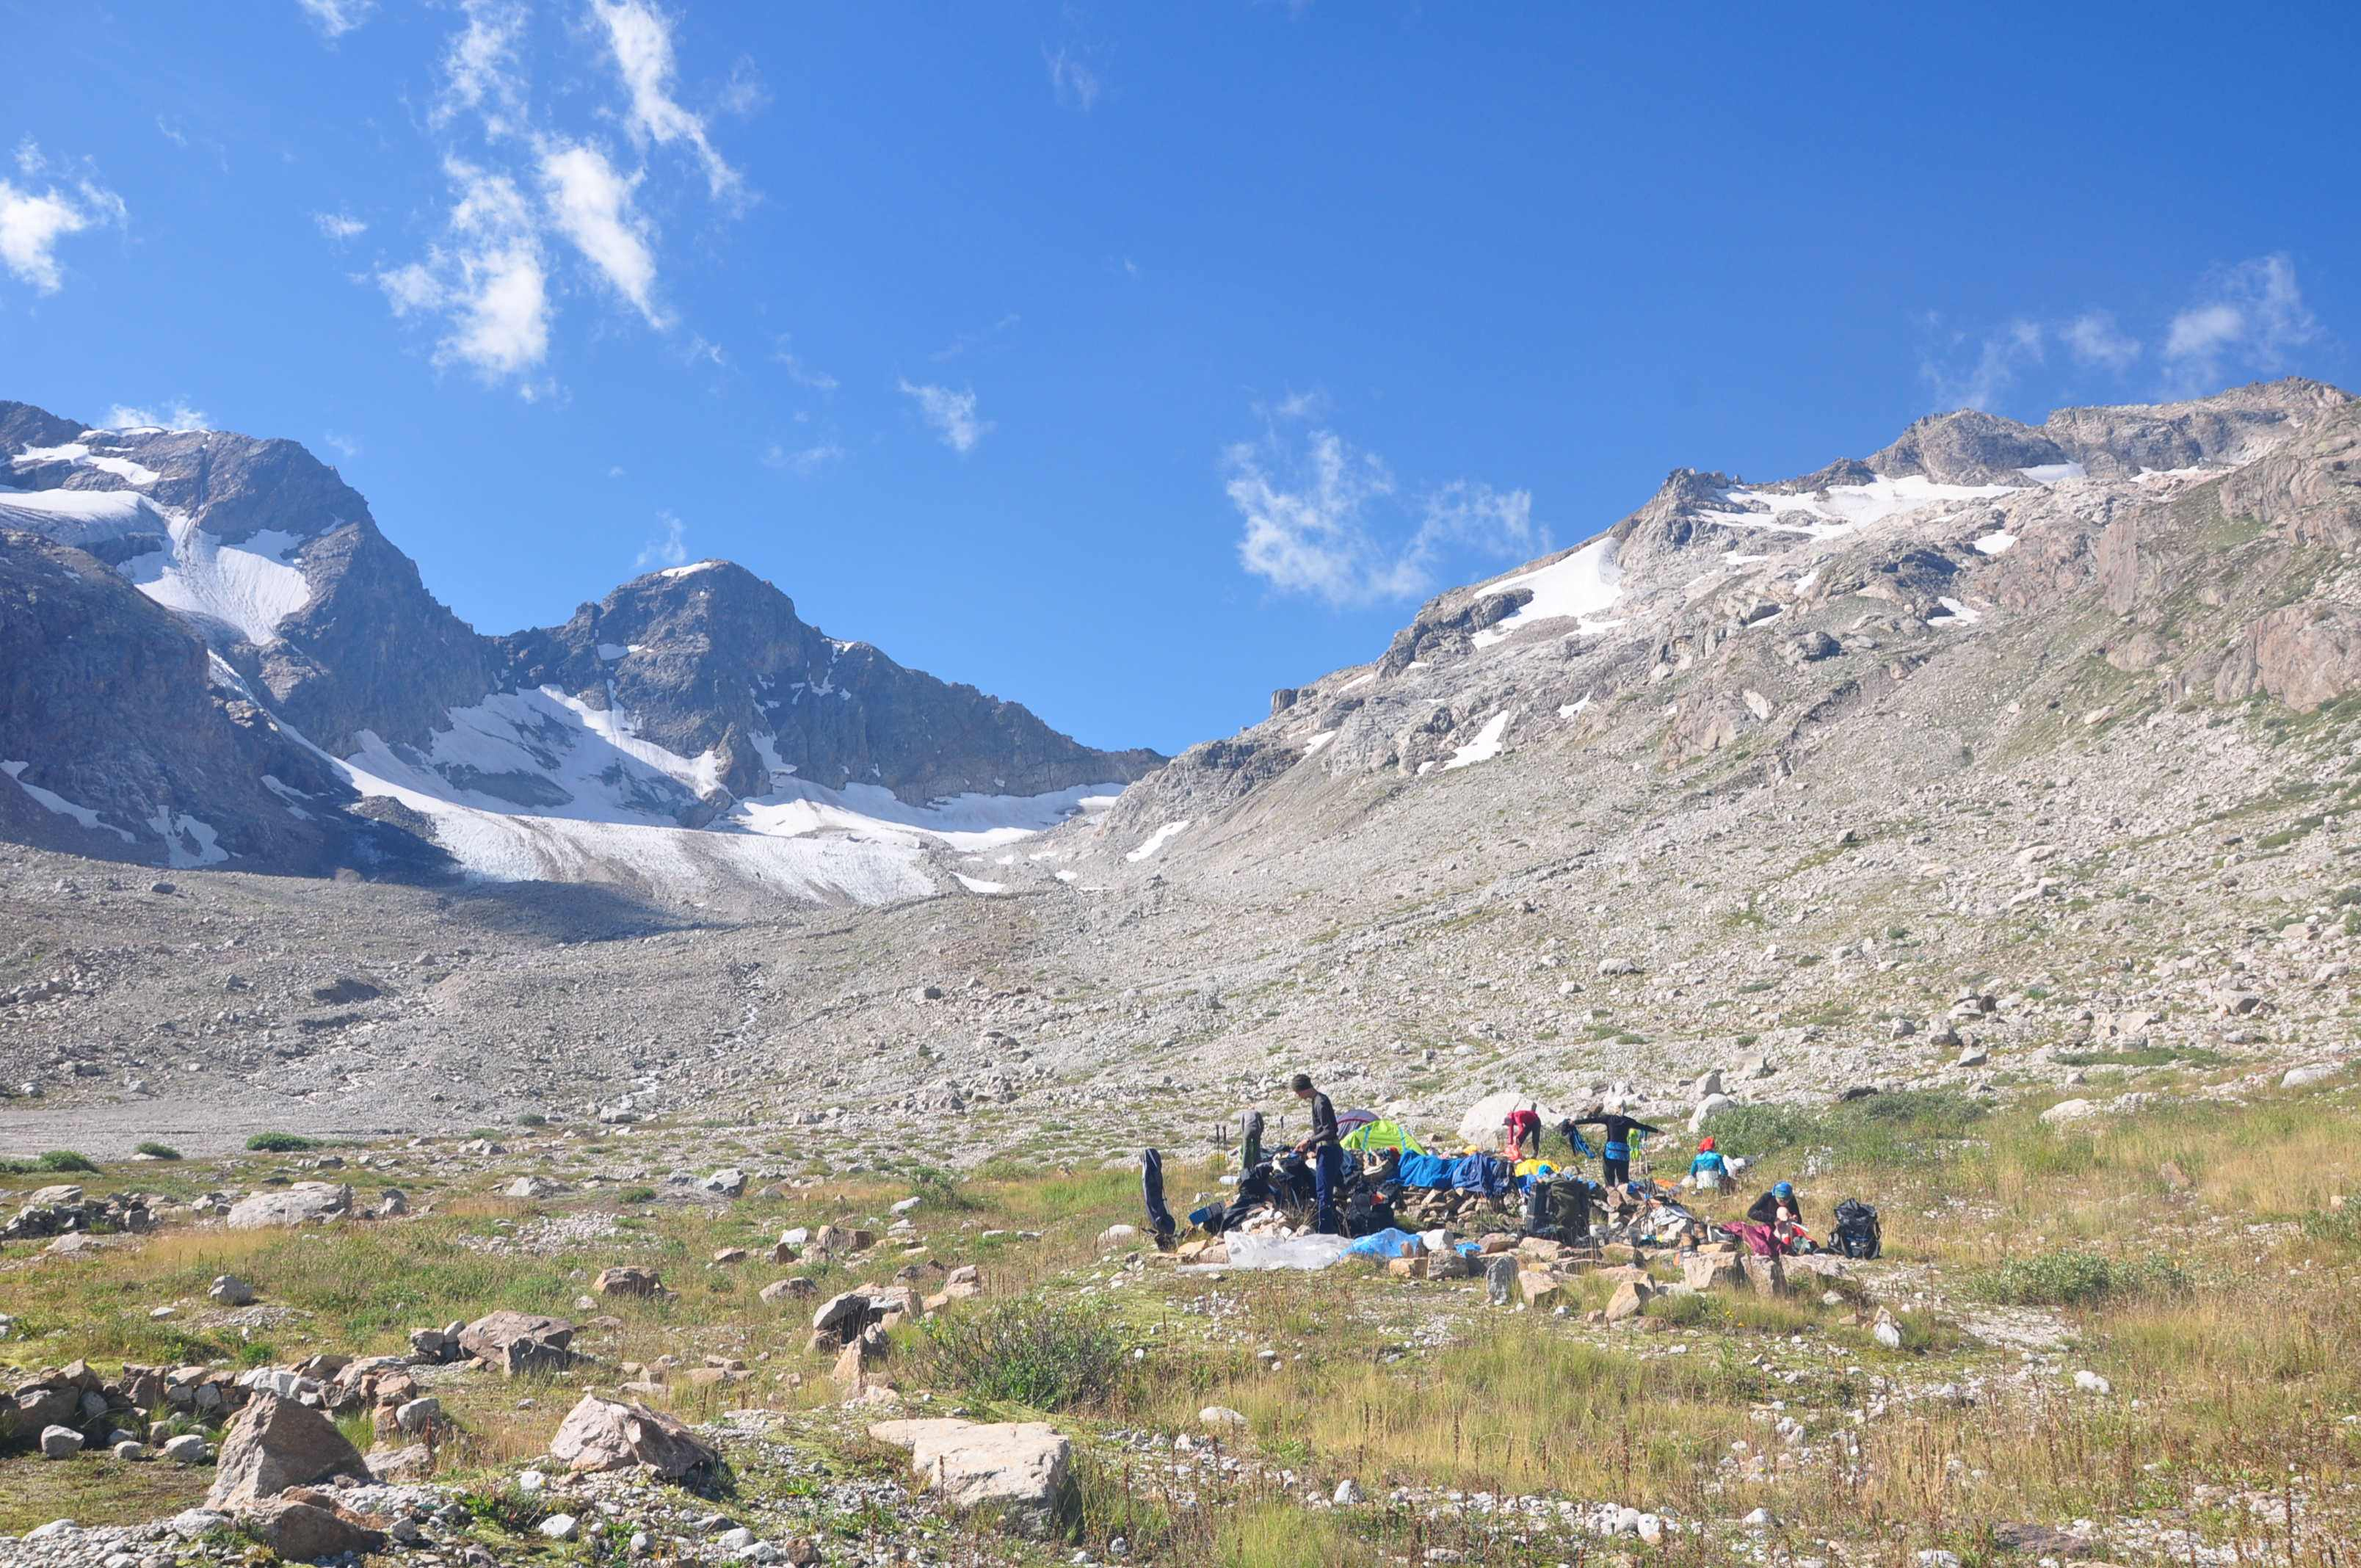
\includegraphics[width=0.7\linewidth]{../pics/DSC_0251.jpg}
	\caption{Утренний лагерь. Активно сушимся.}
	\label{fig:DSC_0251}
\end{figure}

\textbf{Задача номер раз:} перейти многорукавье реки Чунгур-Джар. Есть возможность перебродить реку на урочище Аэродром, при этом некоторые участники могли бы пересечь реку, не замочив ног. Но было принято решение переходить многорукавье реки в верховьях, поднимаясь так, чтобы рукава было можно было перейти посуху всем. Оказалось сложнее, чем казалось. Часть группы всё-таки промочила ботинки и усердно их сушила на каждом привале. 



\begin{figure}[h!]
	\centering
	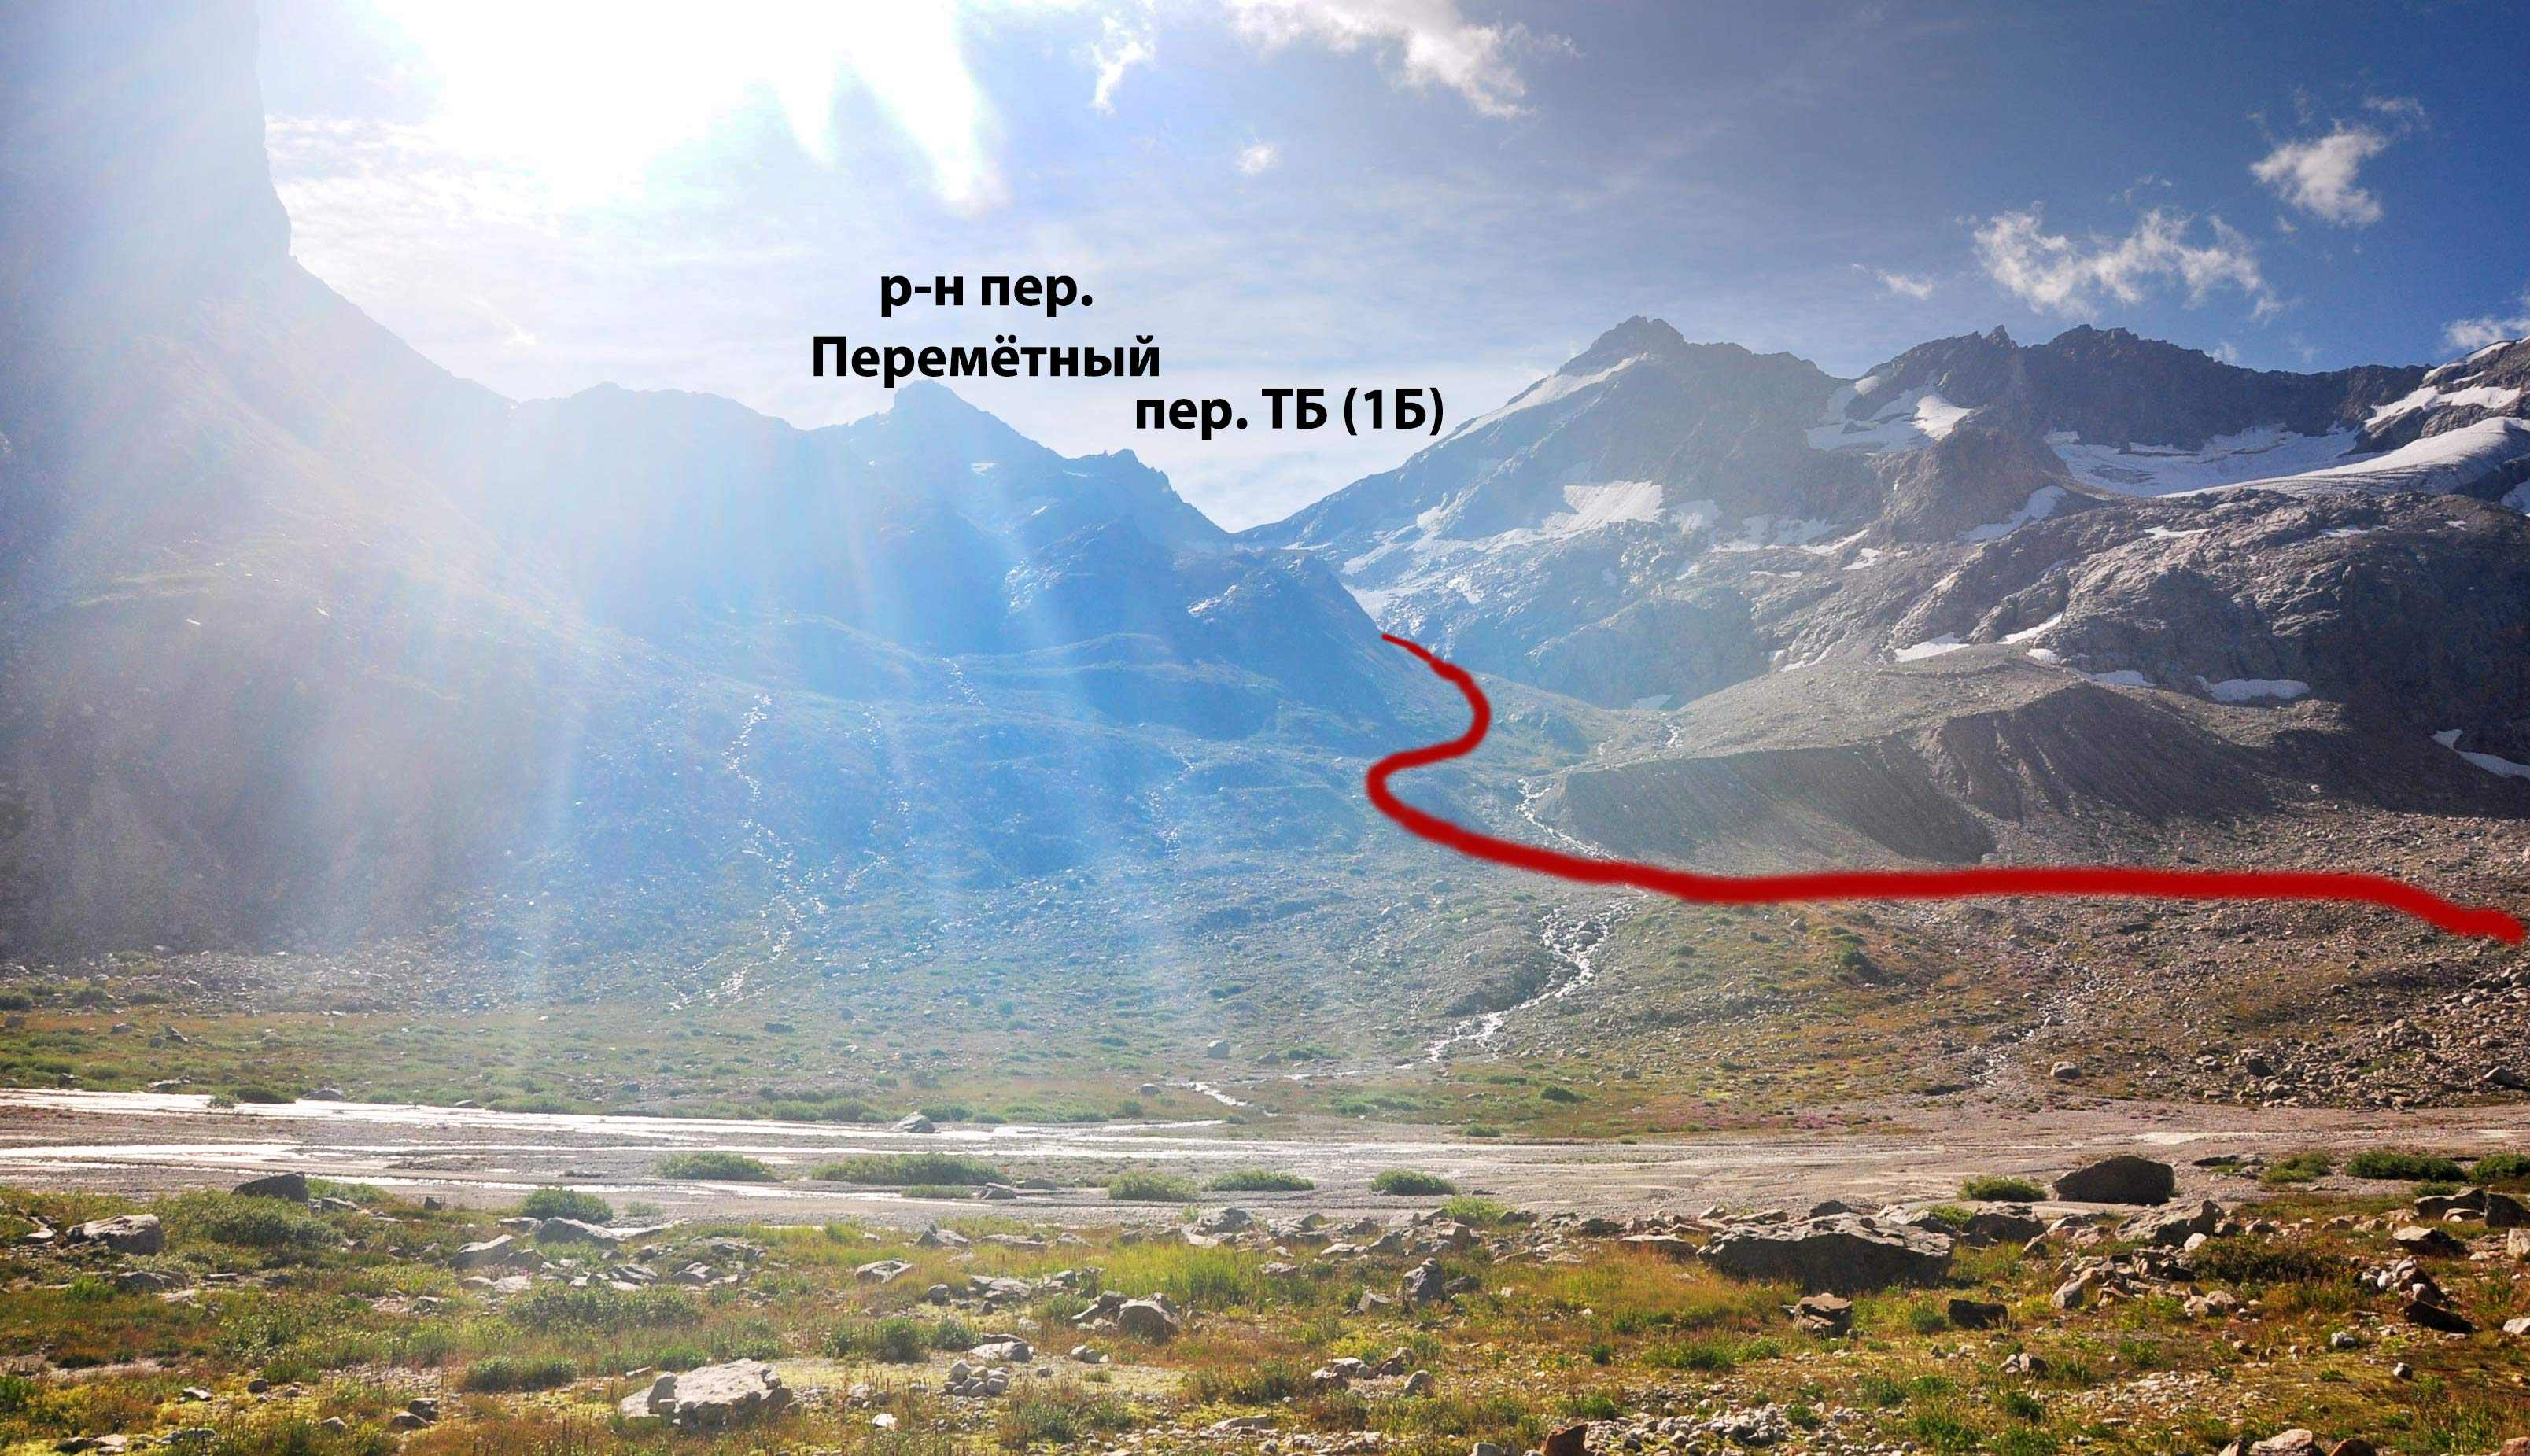
\includegraphics[width=0.7\linewidth]{../pics/DSC_0254.jpg}
	\caption{р. Чунгур-Джар. Нам предстоит перебраться через множество ручейков}
	\label{fig:DSC_0254}
\end{figure}

\begin{figure}[h!]
	\centering
	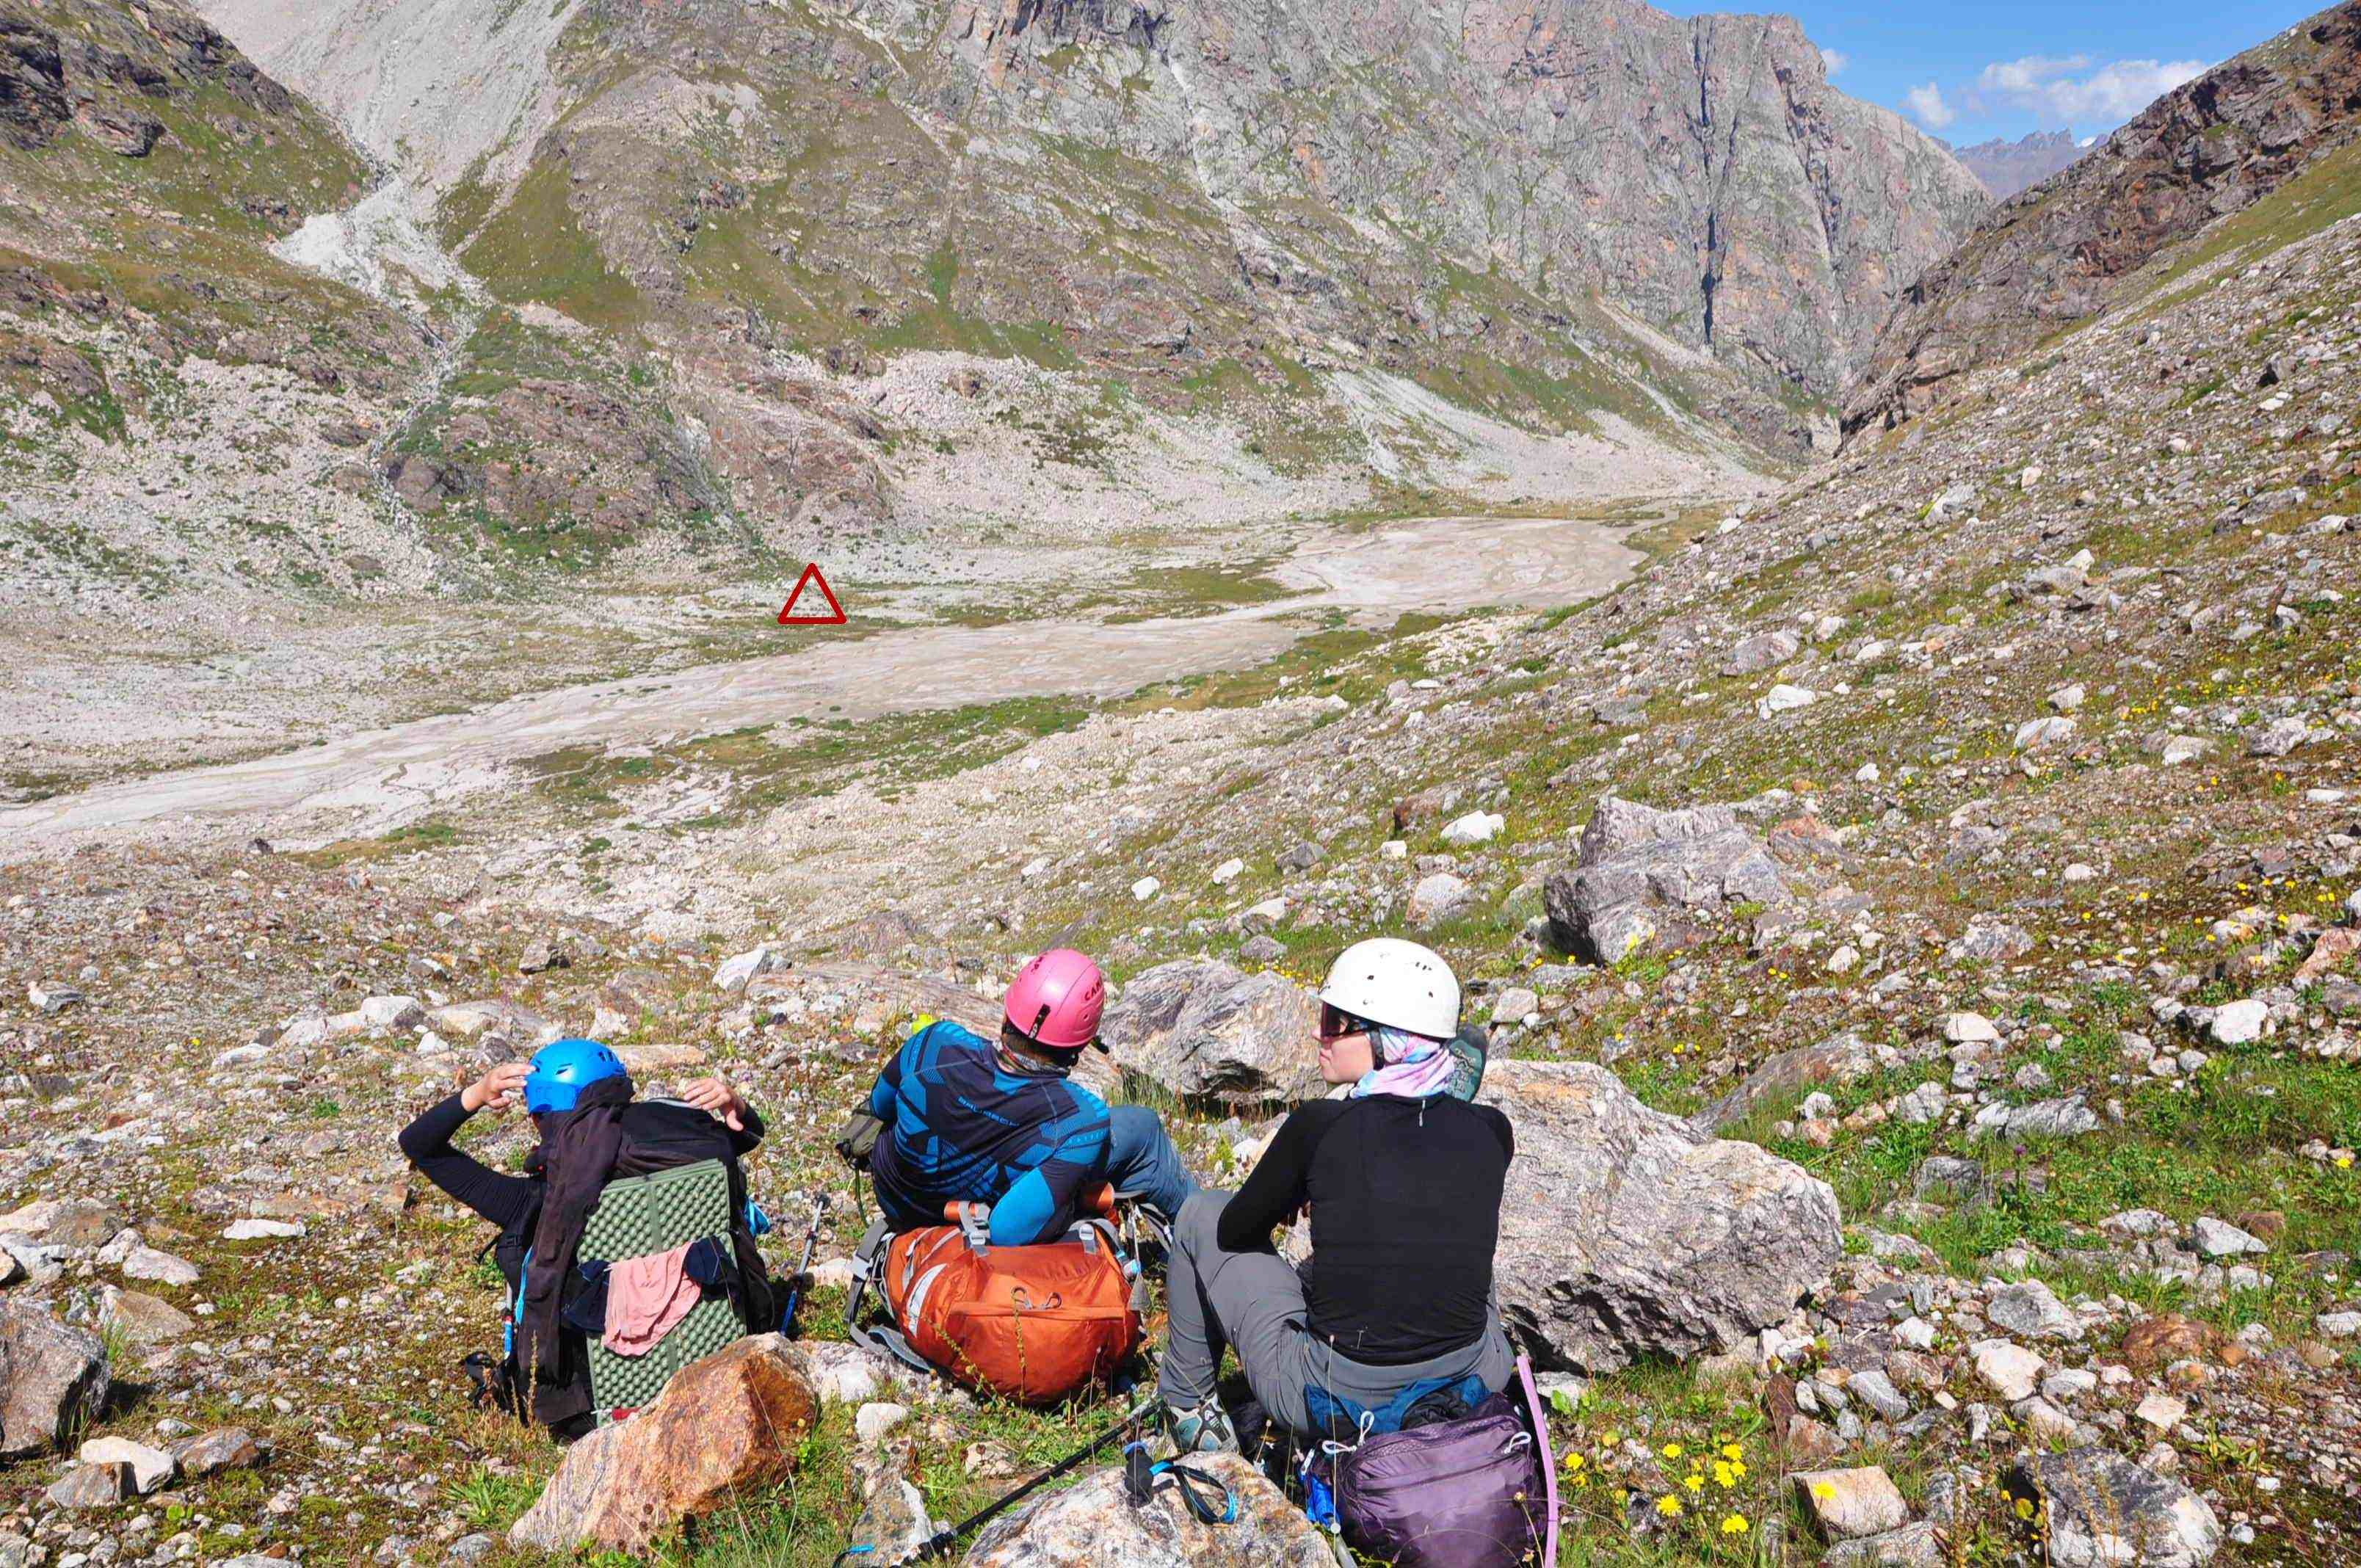
\includegraphics[width=0.7\linewidth]{../pics/DSC_0277.jpg}
	\caption{р. Чунгур-Джар. Перебрались}
	\label{fig:DSC_0277}
\end{figure}


\textbf{Задача номер два:} пройти подъём на перевал. Поднялись на морену по травянисто-каменстому склону, прошли по гребню и попрощались на время с травой. На высоте 2958~м (N43.24135\degree, E42.24827\degree) в 12:33  начали траверс по сыпухе и под небольшой скалой на соседнюю морену (рис.~\ref{fig:perem_1},\ref{fig:DSC_0280}).

\begin{figure}[h!]
	\centering
	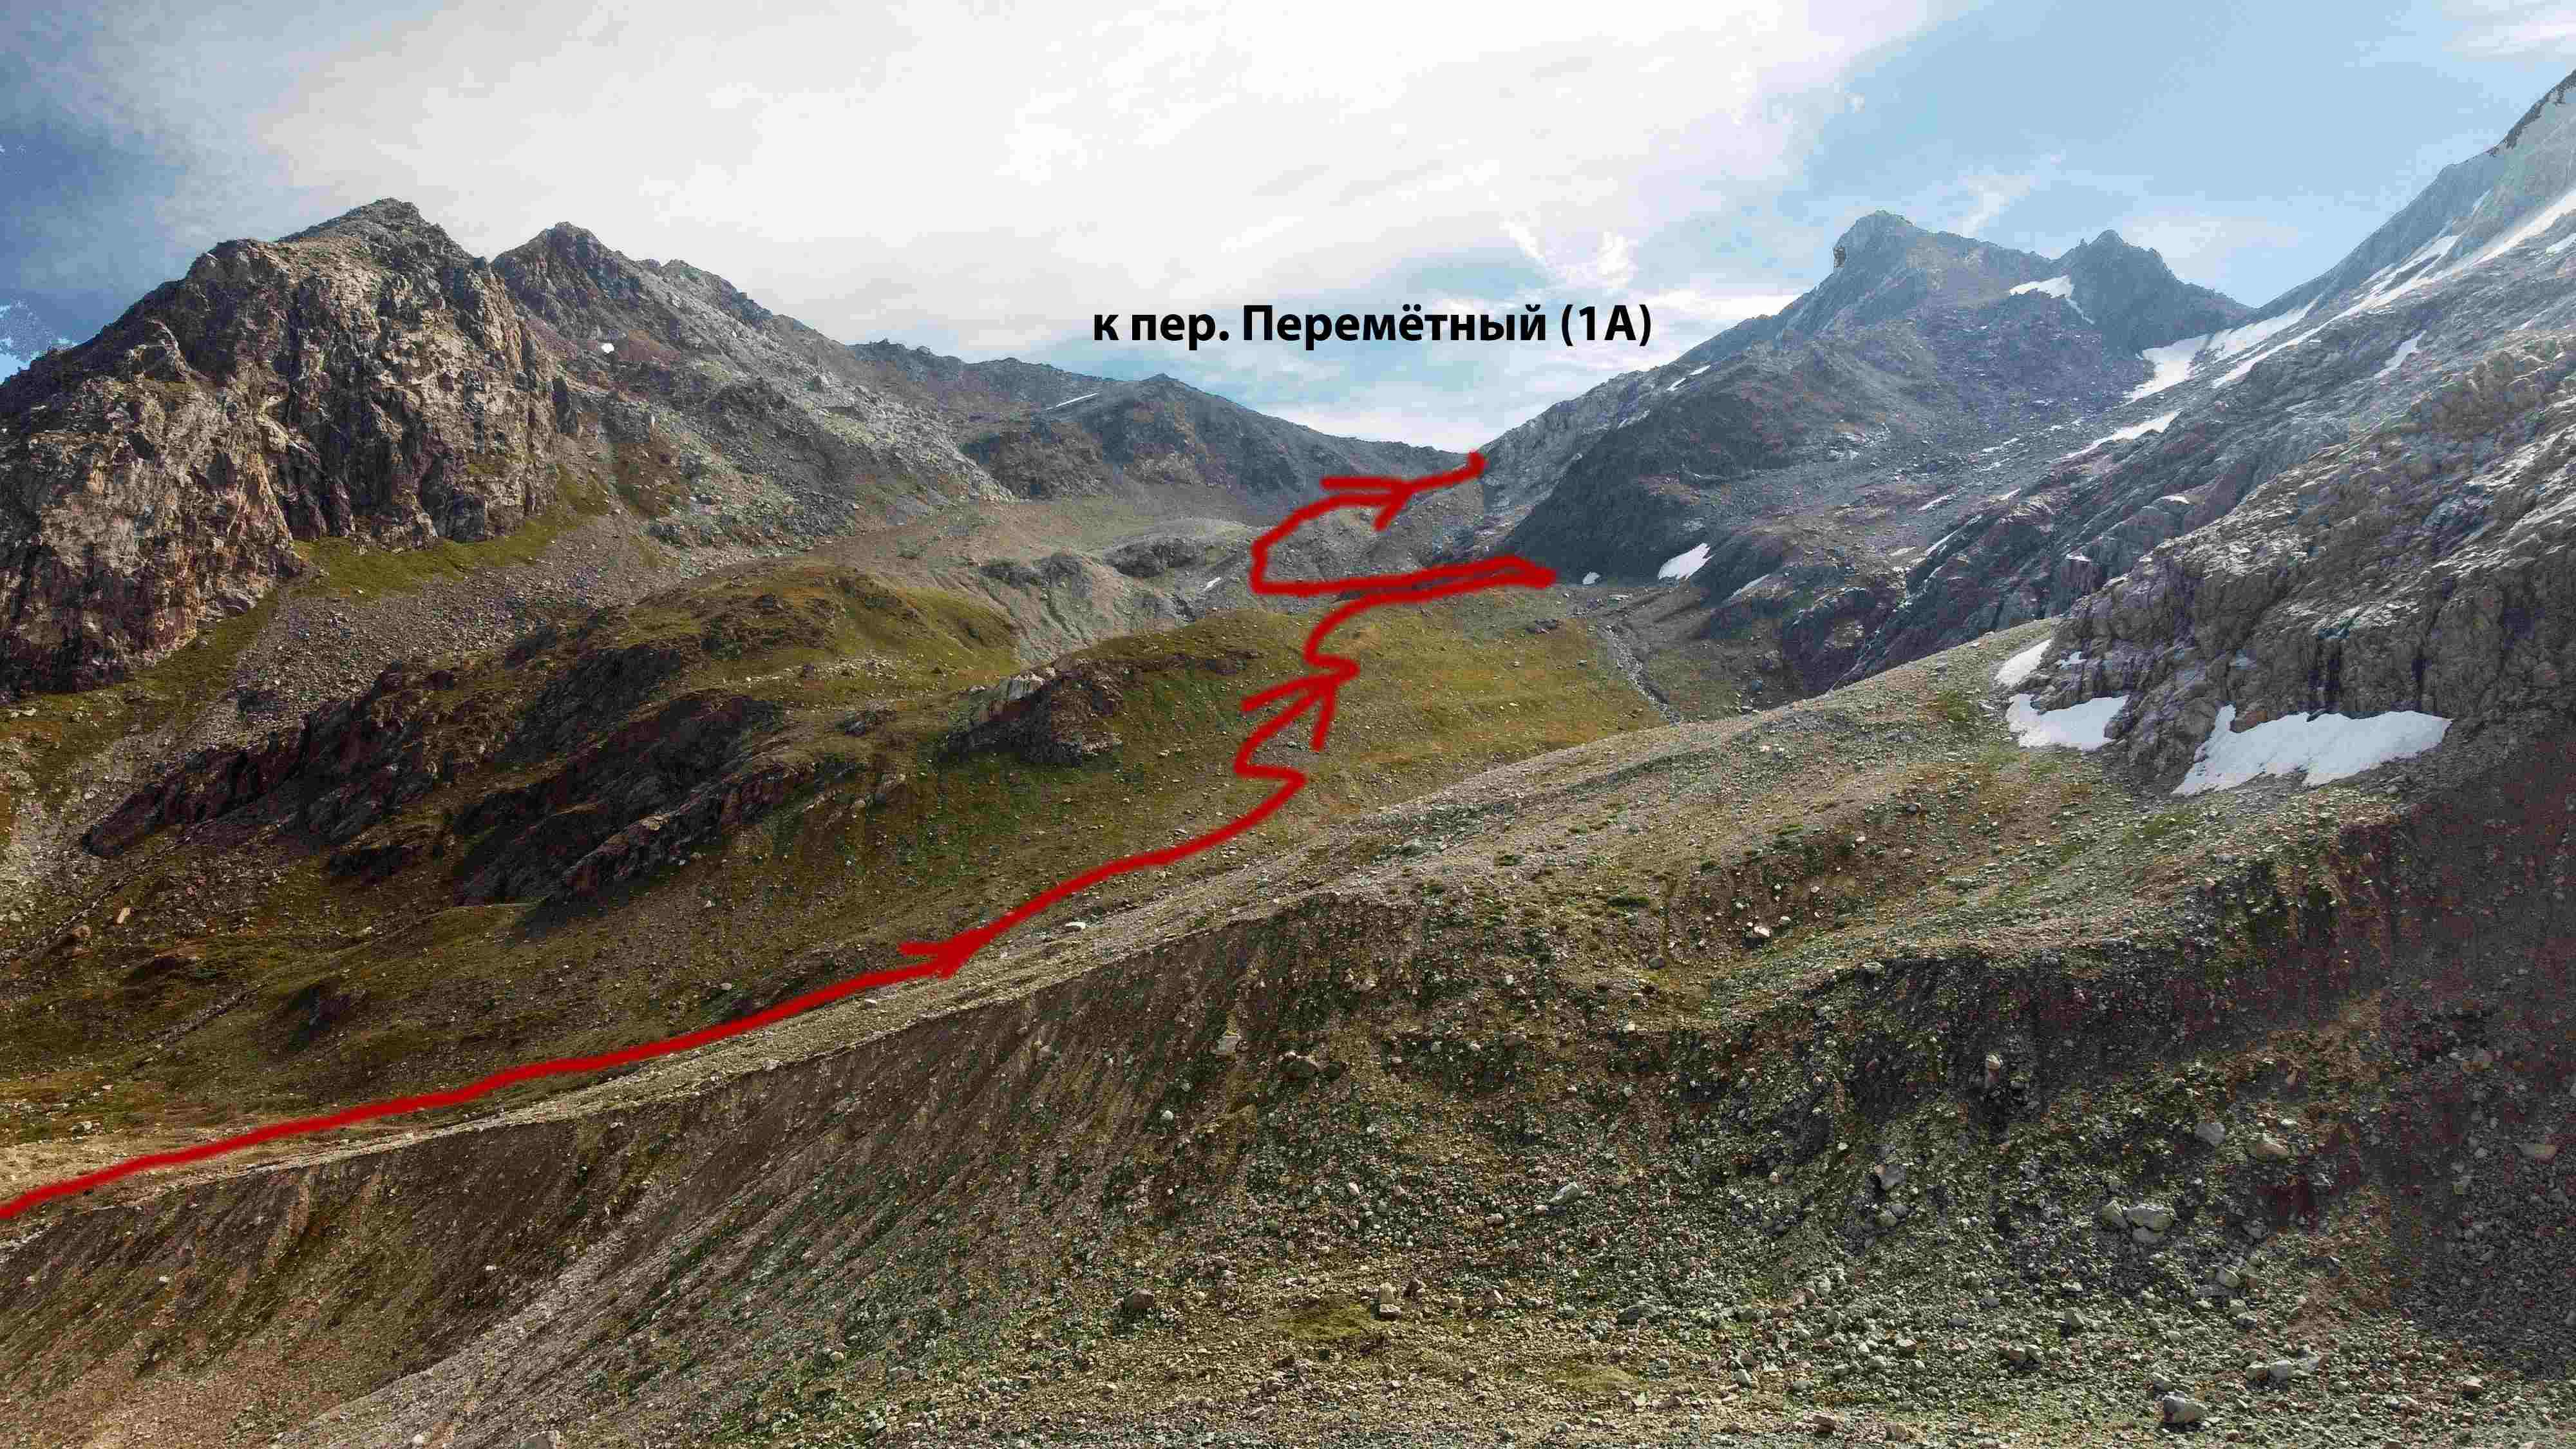
\includegraphics[width=0.7\linewidth]{../pics/perem_1}
	\caption{Начало подъёма к пер. Перемётный из д.р. Чунгур-Джар}
	\label{fig:perem_1}
\end{figure} 
\begin{figure}[h!]
	\centering
	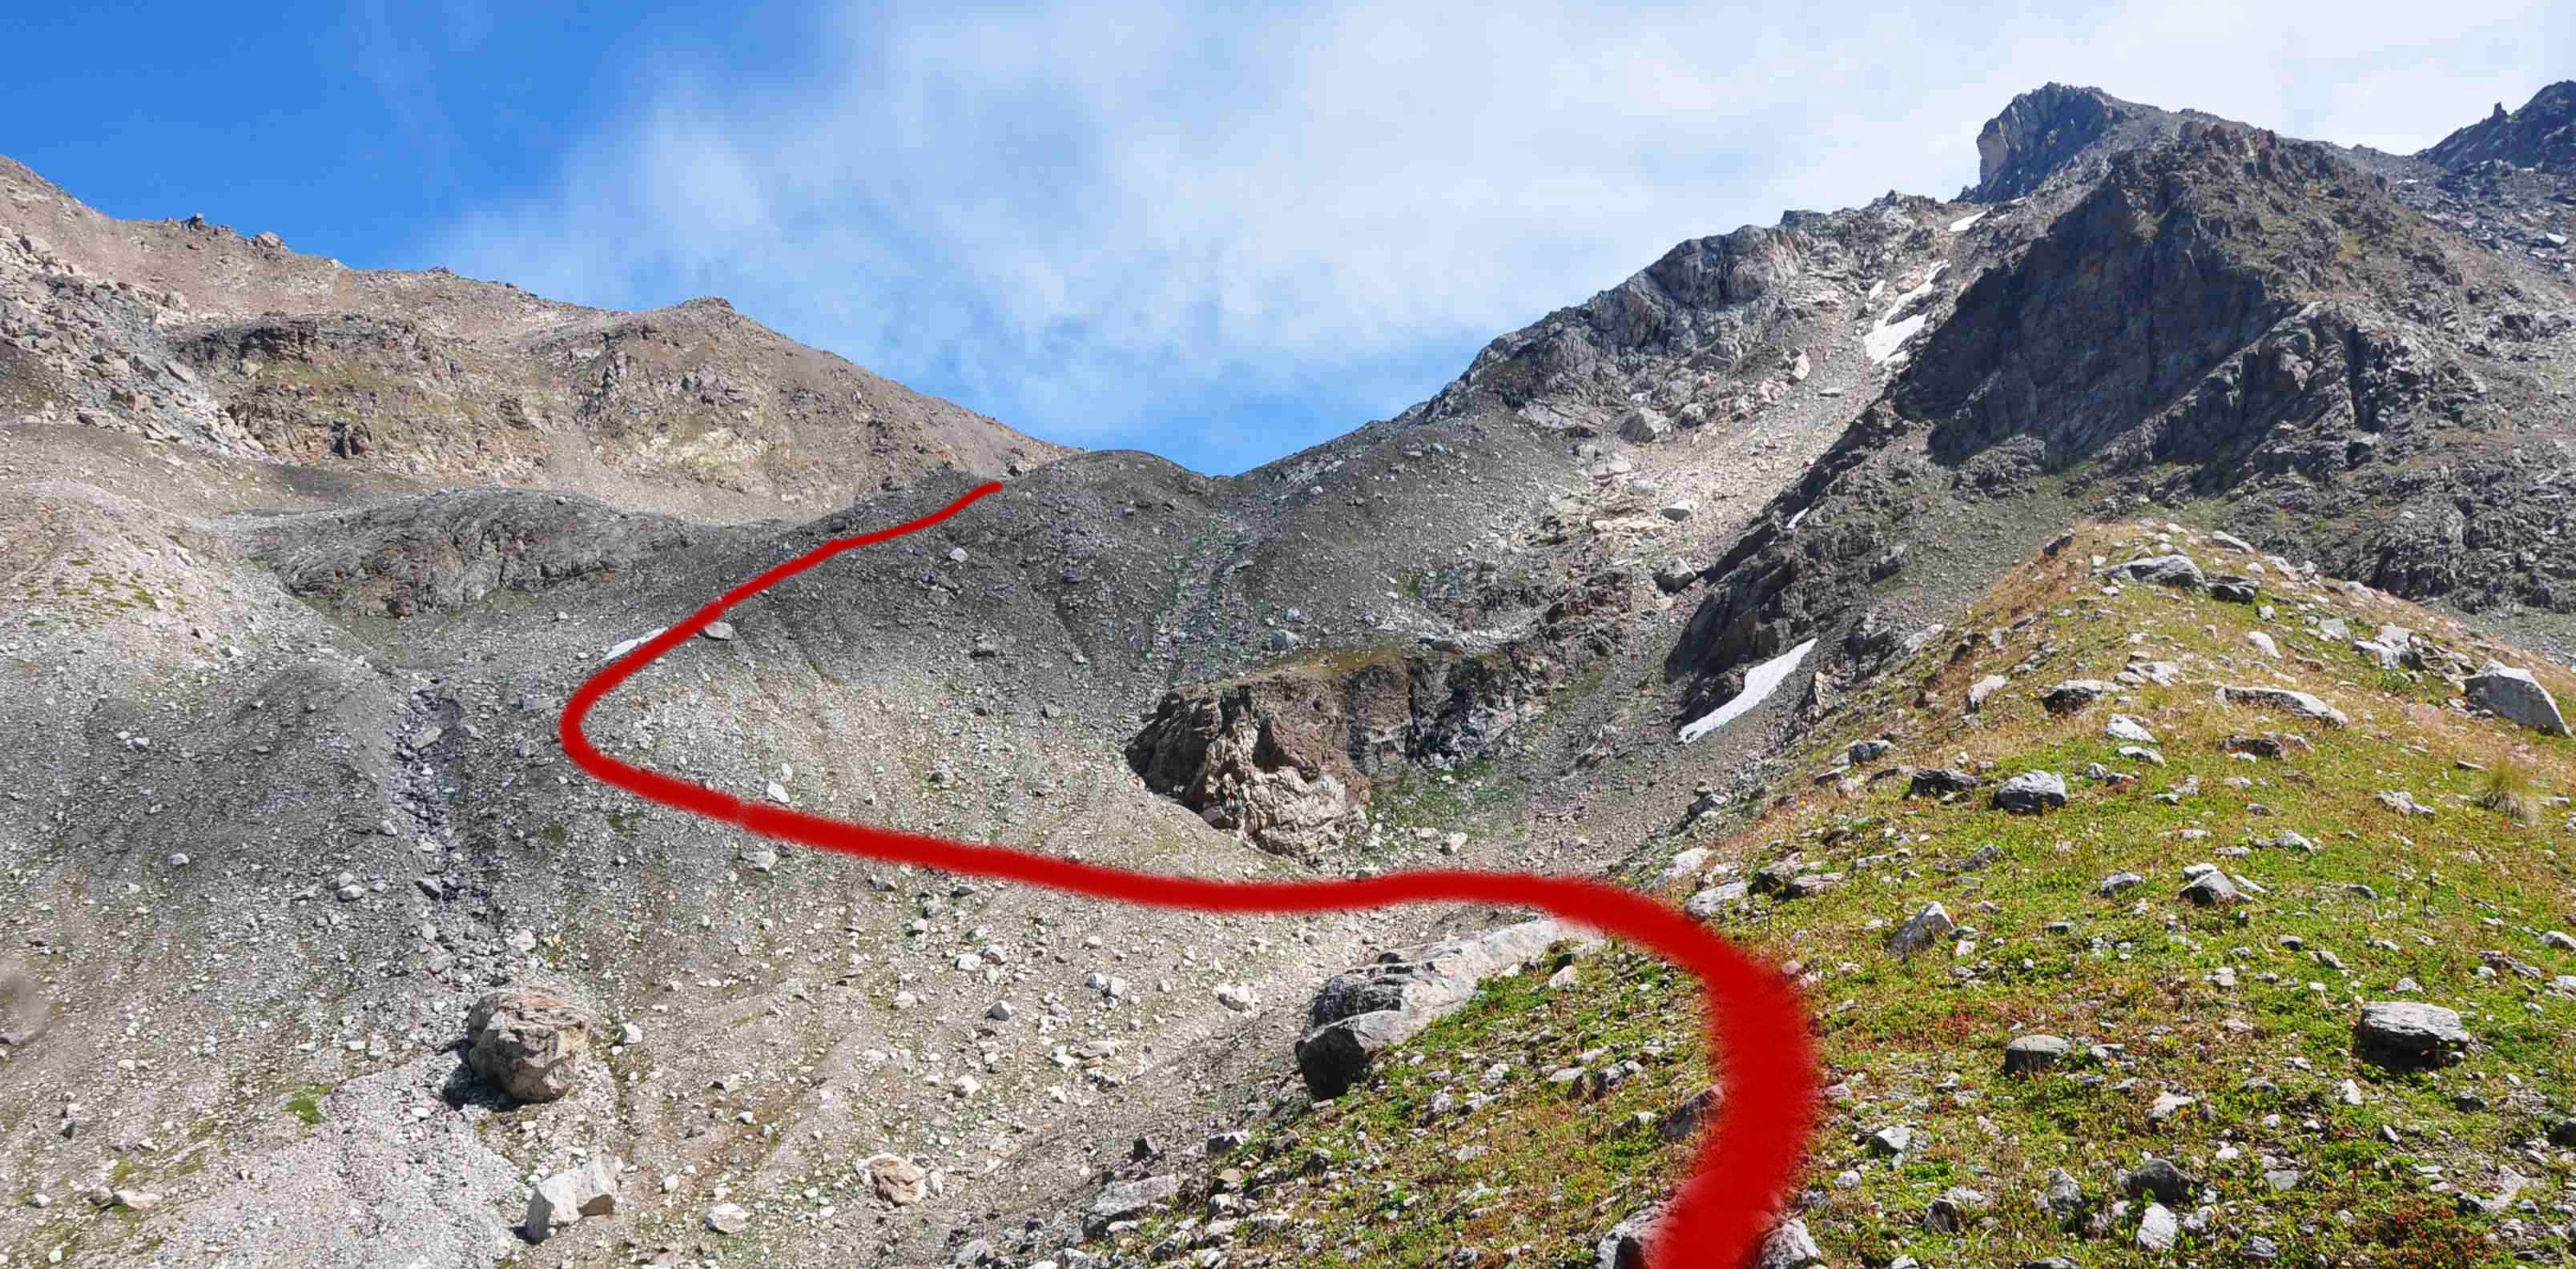
\includegraphics[width=0.7\linewidth]{../pics/DSC_0280.jpg}
	\caption{Траверс по моренам и выход на  моренный гребень}
	\label{fig:DSC_0280}
\end{figure} 


После этого~--- прямым курсом на перевал. Финальный участок подъёма идёт по пологой средней осыпи и не является трудным ни физически, ни технически, ни психологически (рис.~\ref{fig:DSC_0341}).
\begin{figure}[h!]
	\centering
	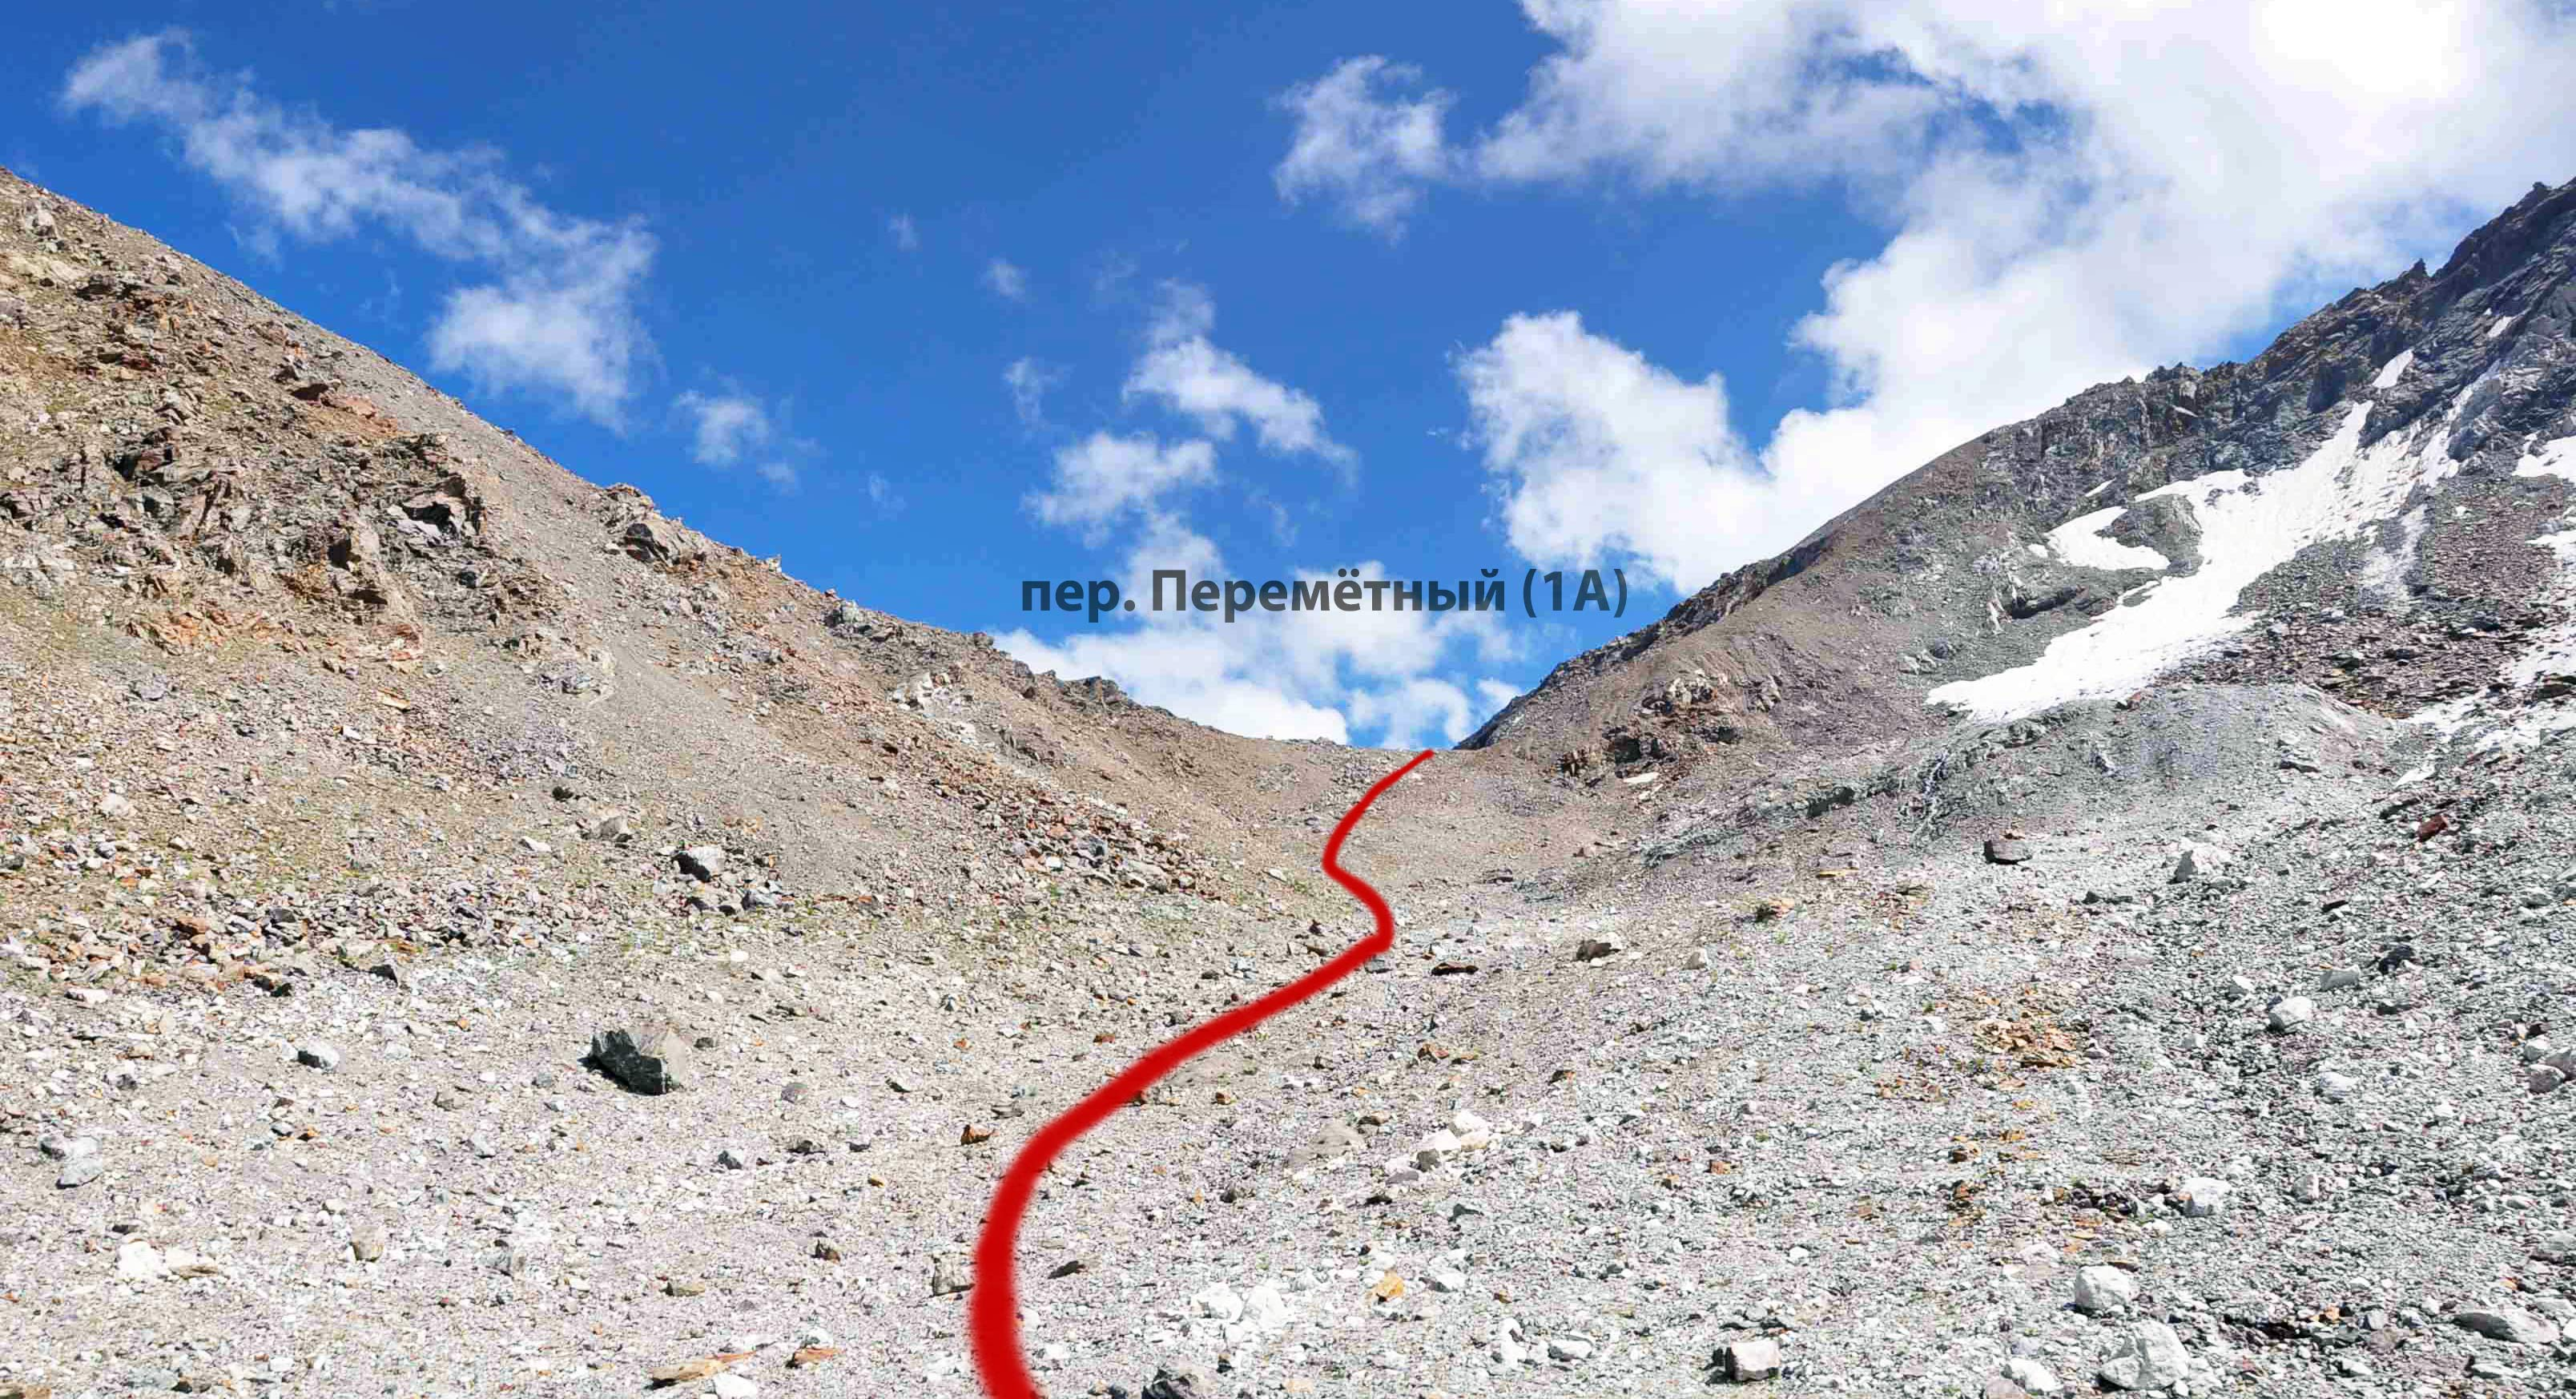
\includegraphics[width=0.7\linewidth]{../pics/DSC_0341.jpg}
	\caption{Перевальный взлёт}
	\label{fig:DSC_0341}
\end{figure} 

С задачей два справились в 14:33 (рис.~\ref{fig:DSC_0412}). На перевале сняли записку группы туристов из Ростова-на-Дону и Новочеркасска от 20.08.2019 (рис.~\ref{pic:peremetnyy}). Примечательно, что эта группа в своё время сняла записку Горной секции МФТИ под руководством Королёва Андрея от 2018 года~--- в этот поход ходила руковод.

\begin{figure}[h!]
	\centering
	\begin{minipage}[h]{0.55\linewidth}
		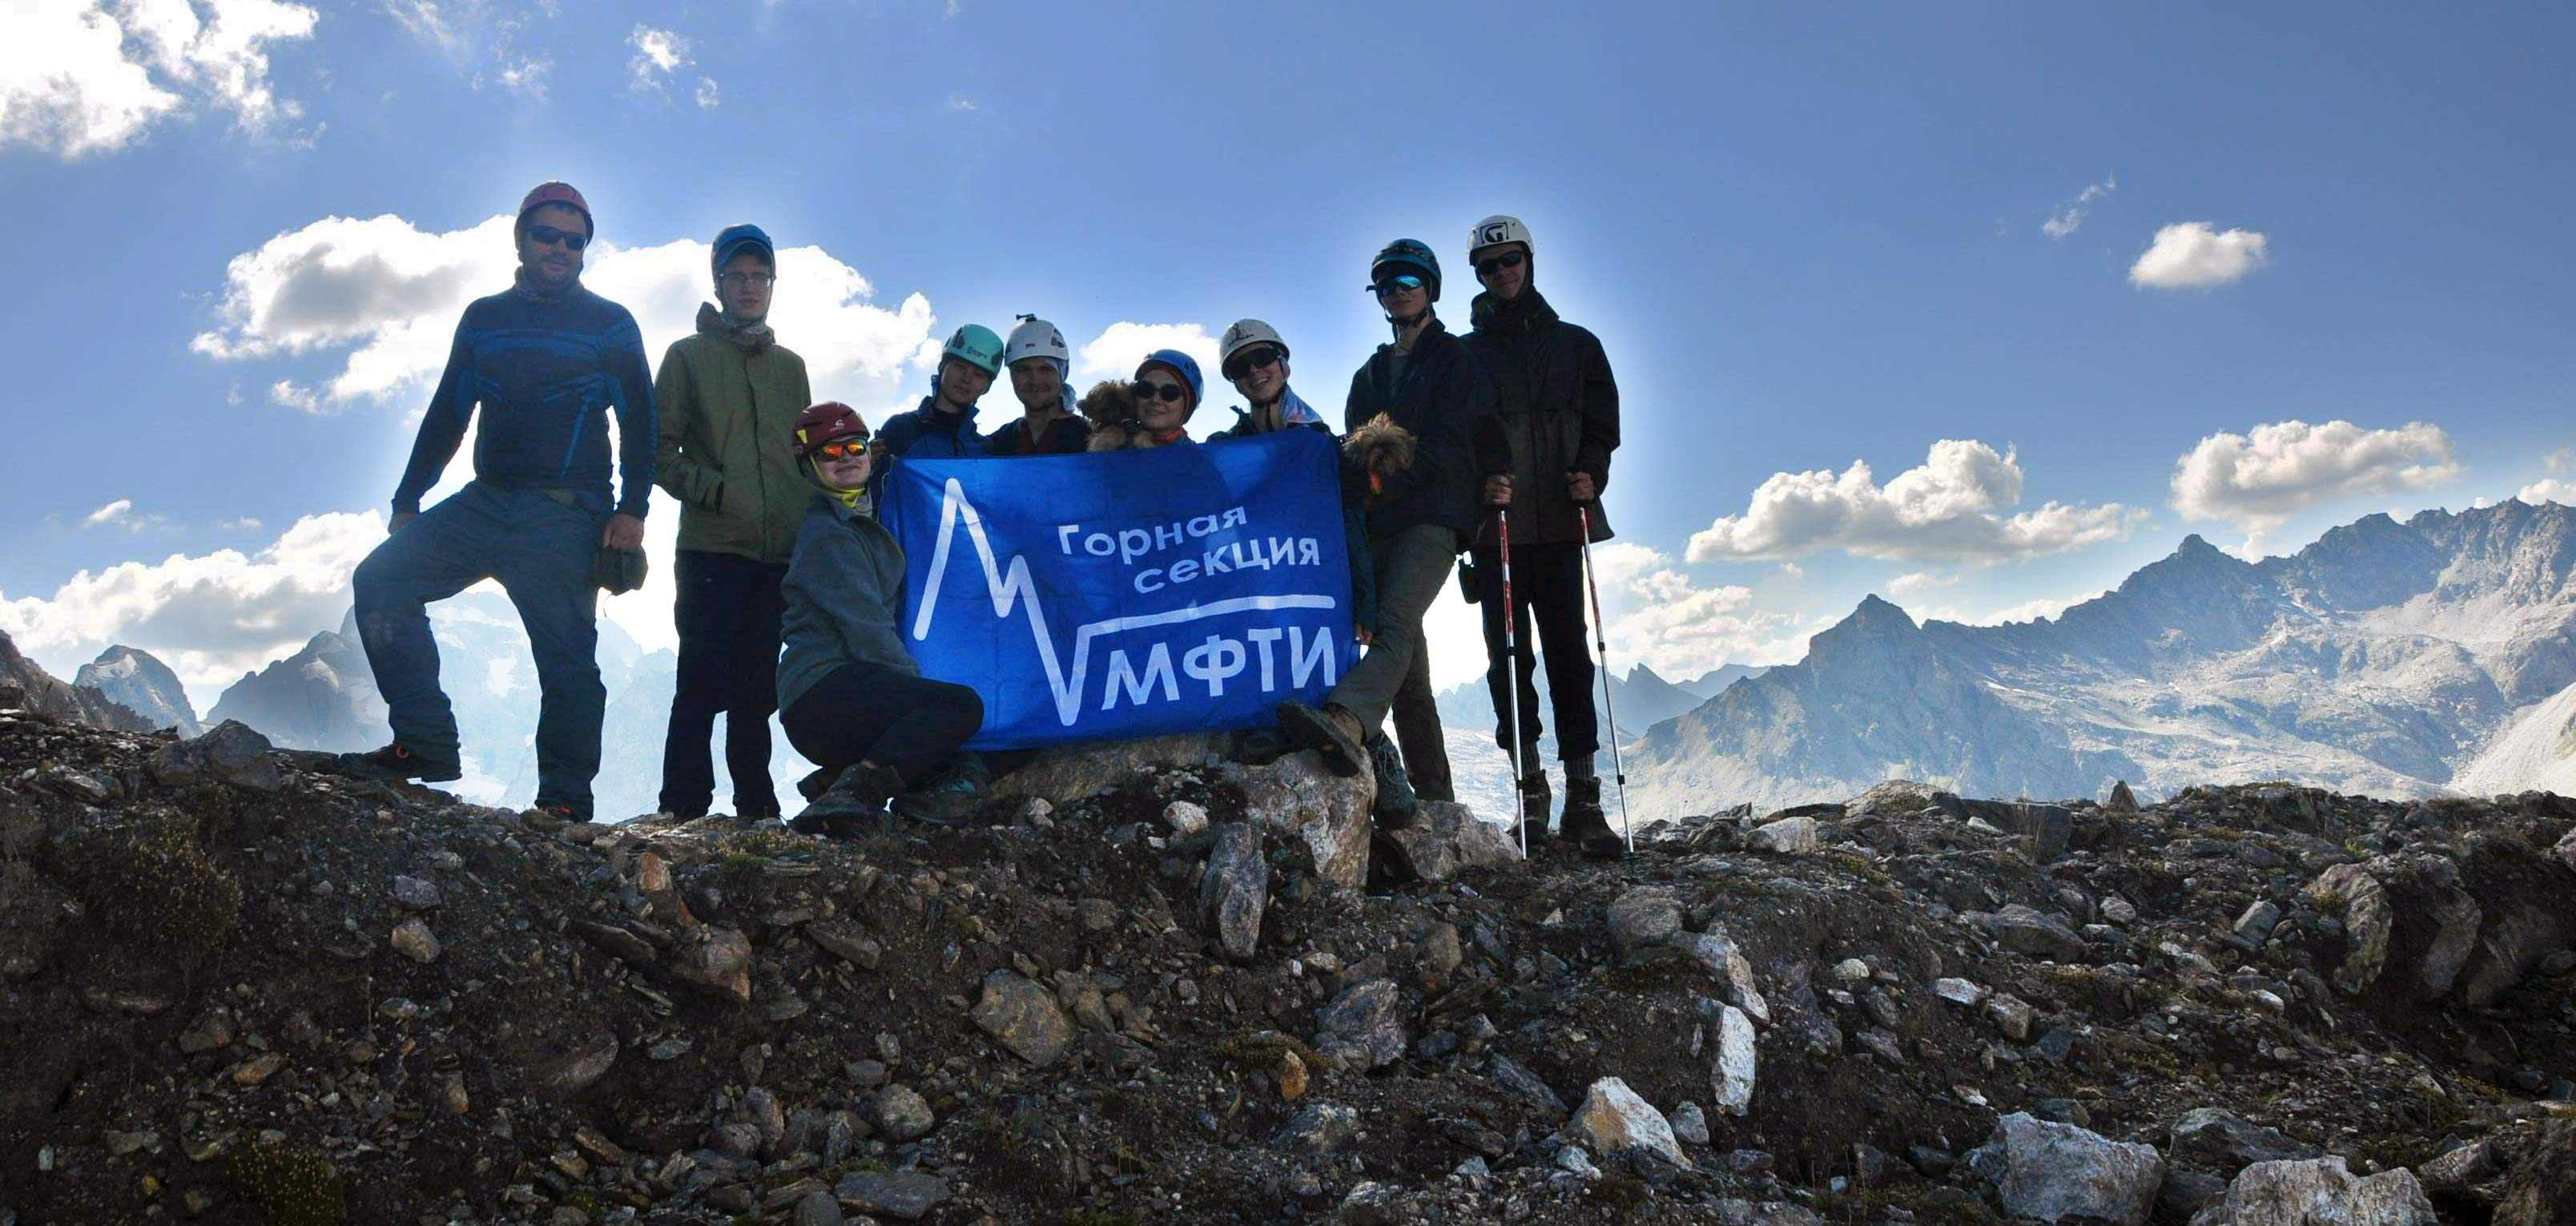
\includegraphics[width=0.99\linewidth]{../pics/DSC_0412 2.jpg}
	\end{minipage}
	\hfill
	\begin{minipage}[h]{0.45\linewidth}
		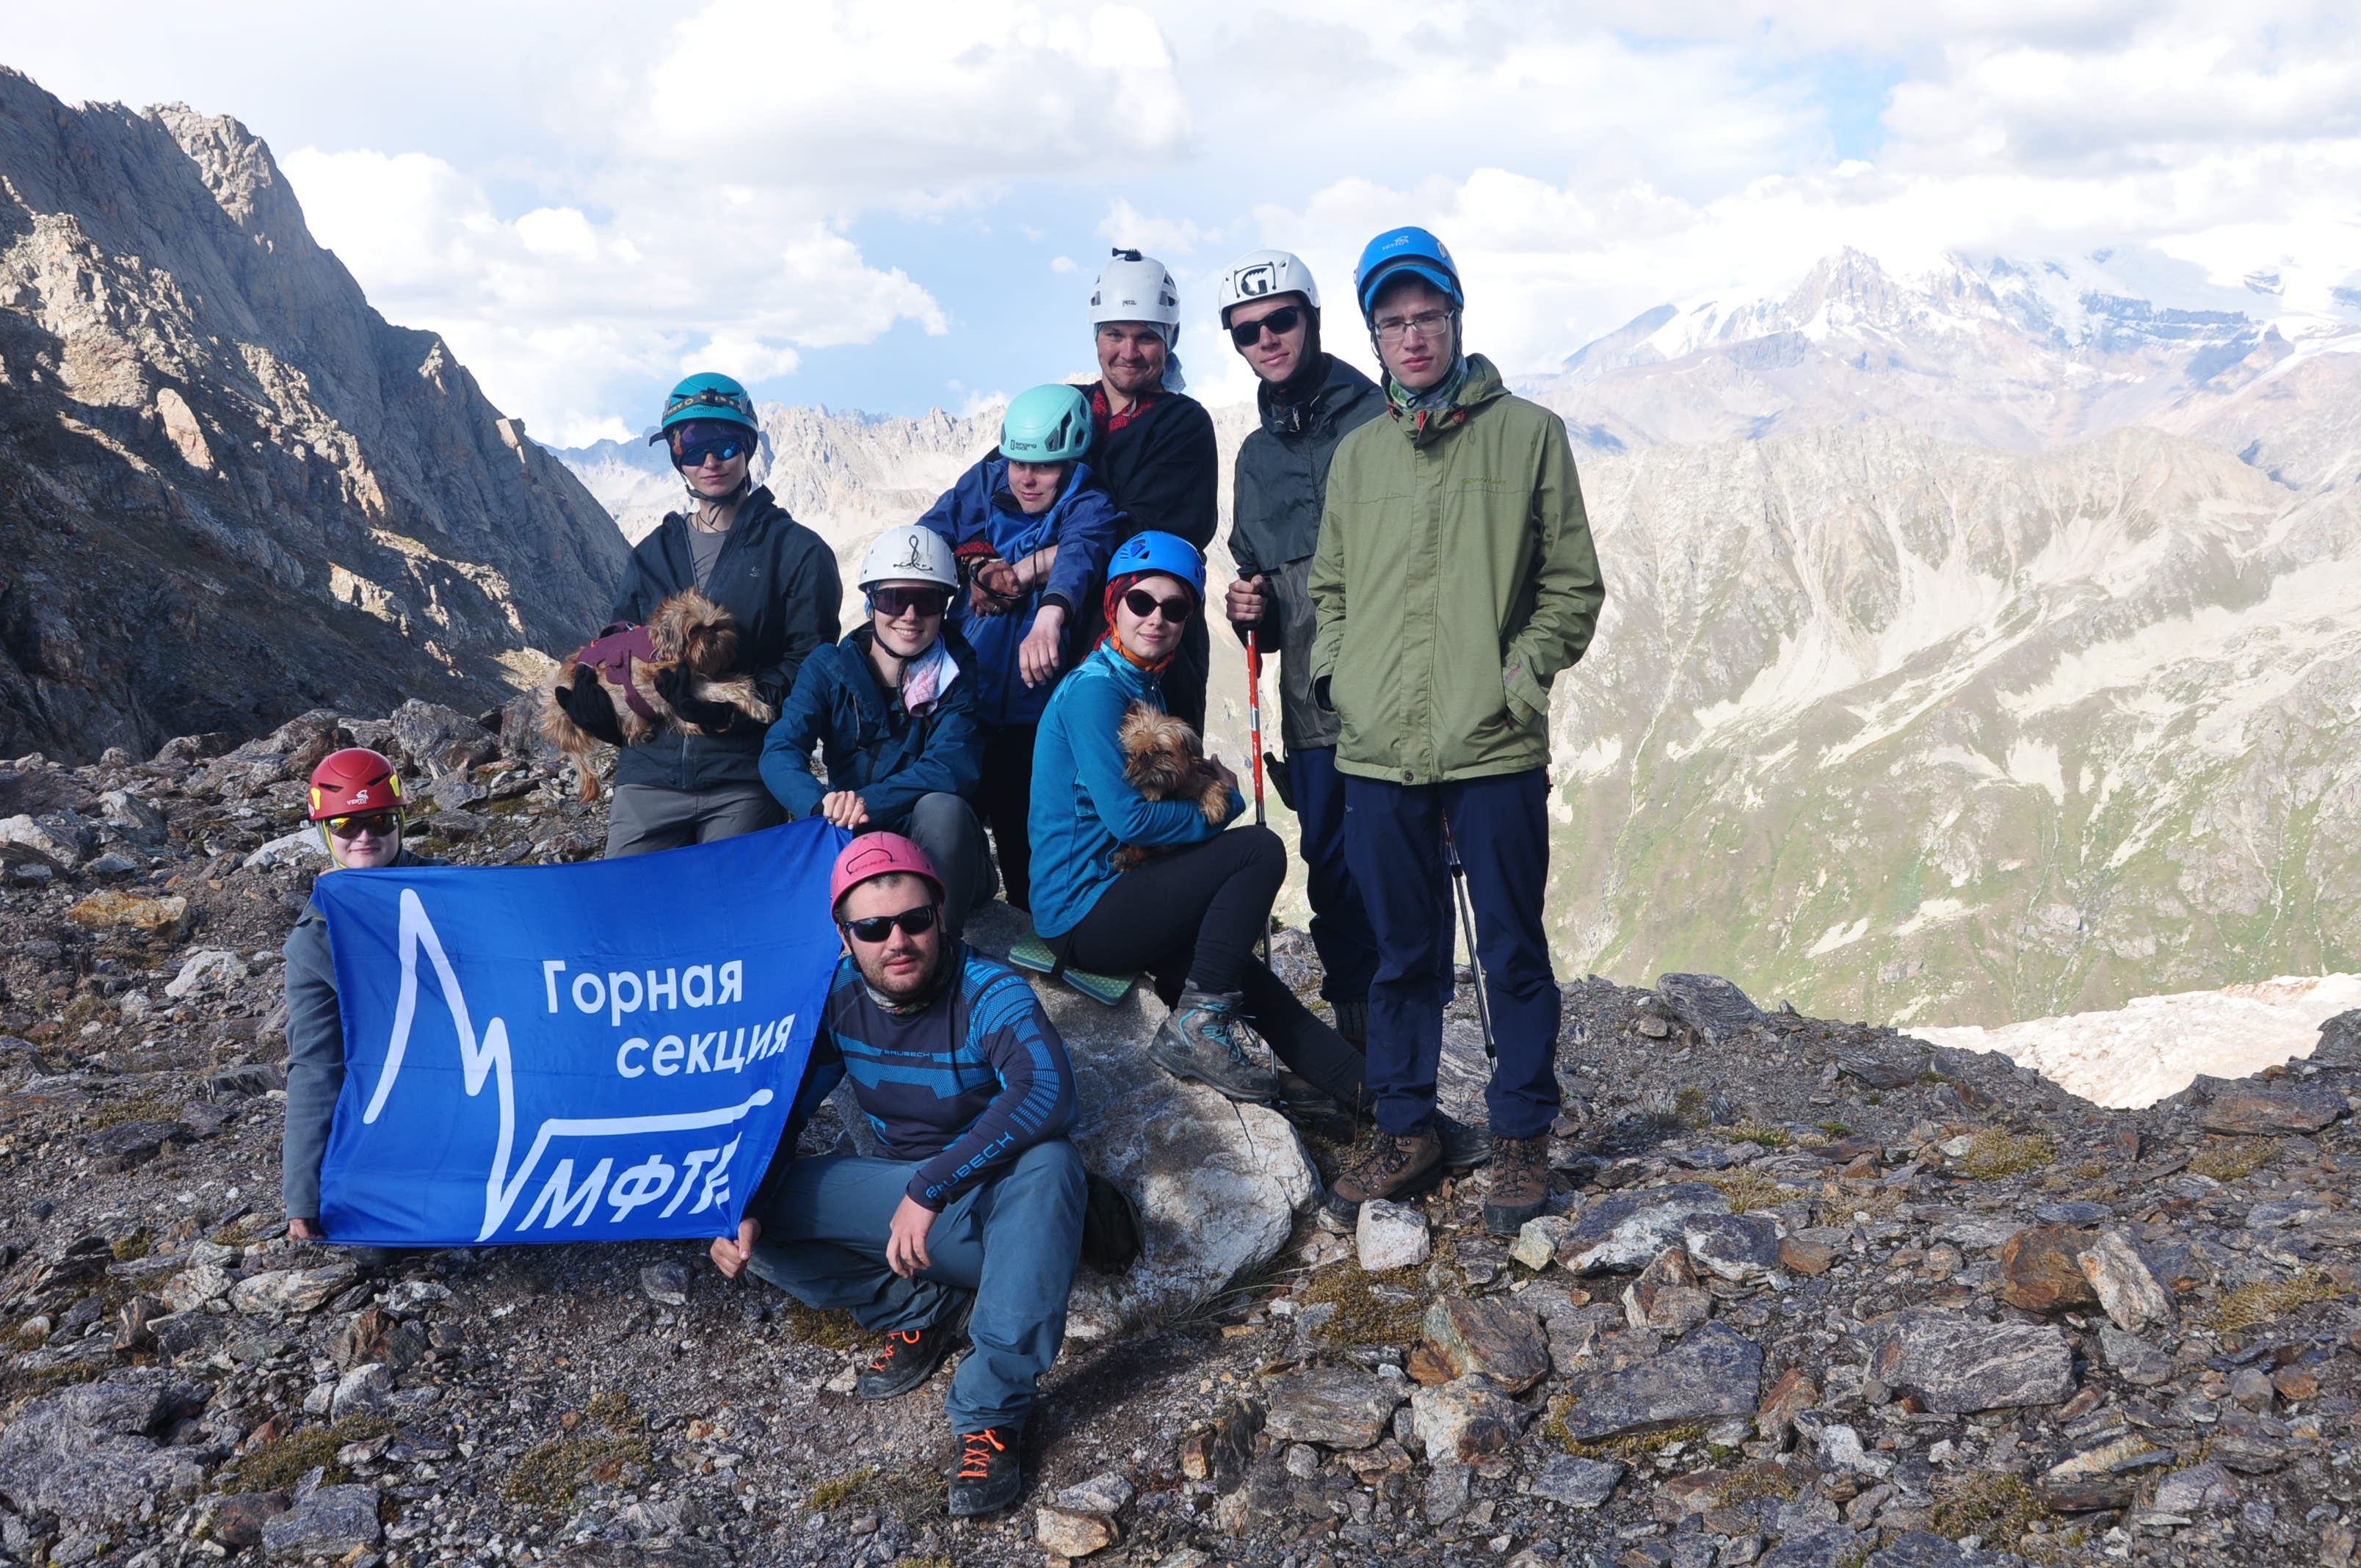
\includegraphics[width=0.99\linewidth]{../pics/DSC_0419 2.jpg}
	\end{minipage}
	\caption{Группа на пер. Перемётный. Слева: вид в д.р. Чунгур-Джар, справа: вид в д.р. Танышхан}
	\label{fig:DSC_0412}
\end{figure}


\begin{figure}[h!]
	\centering
	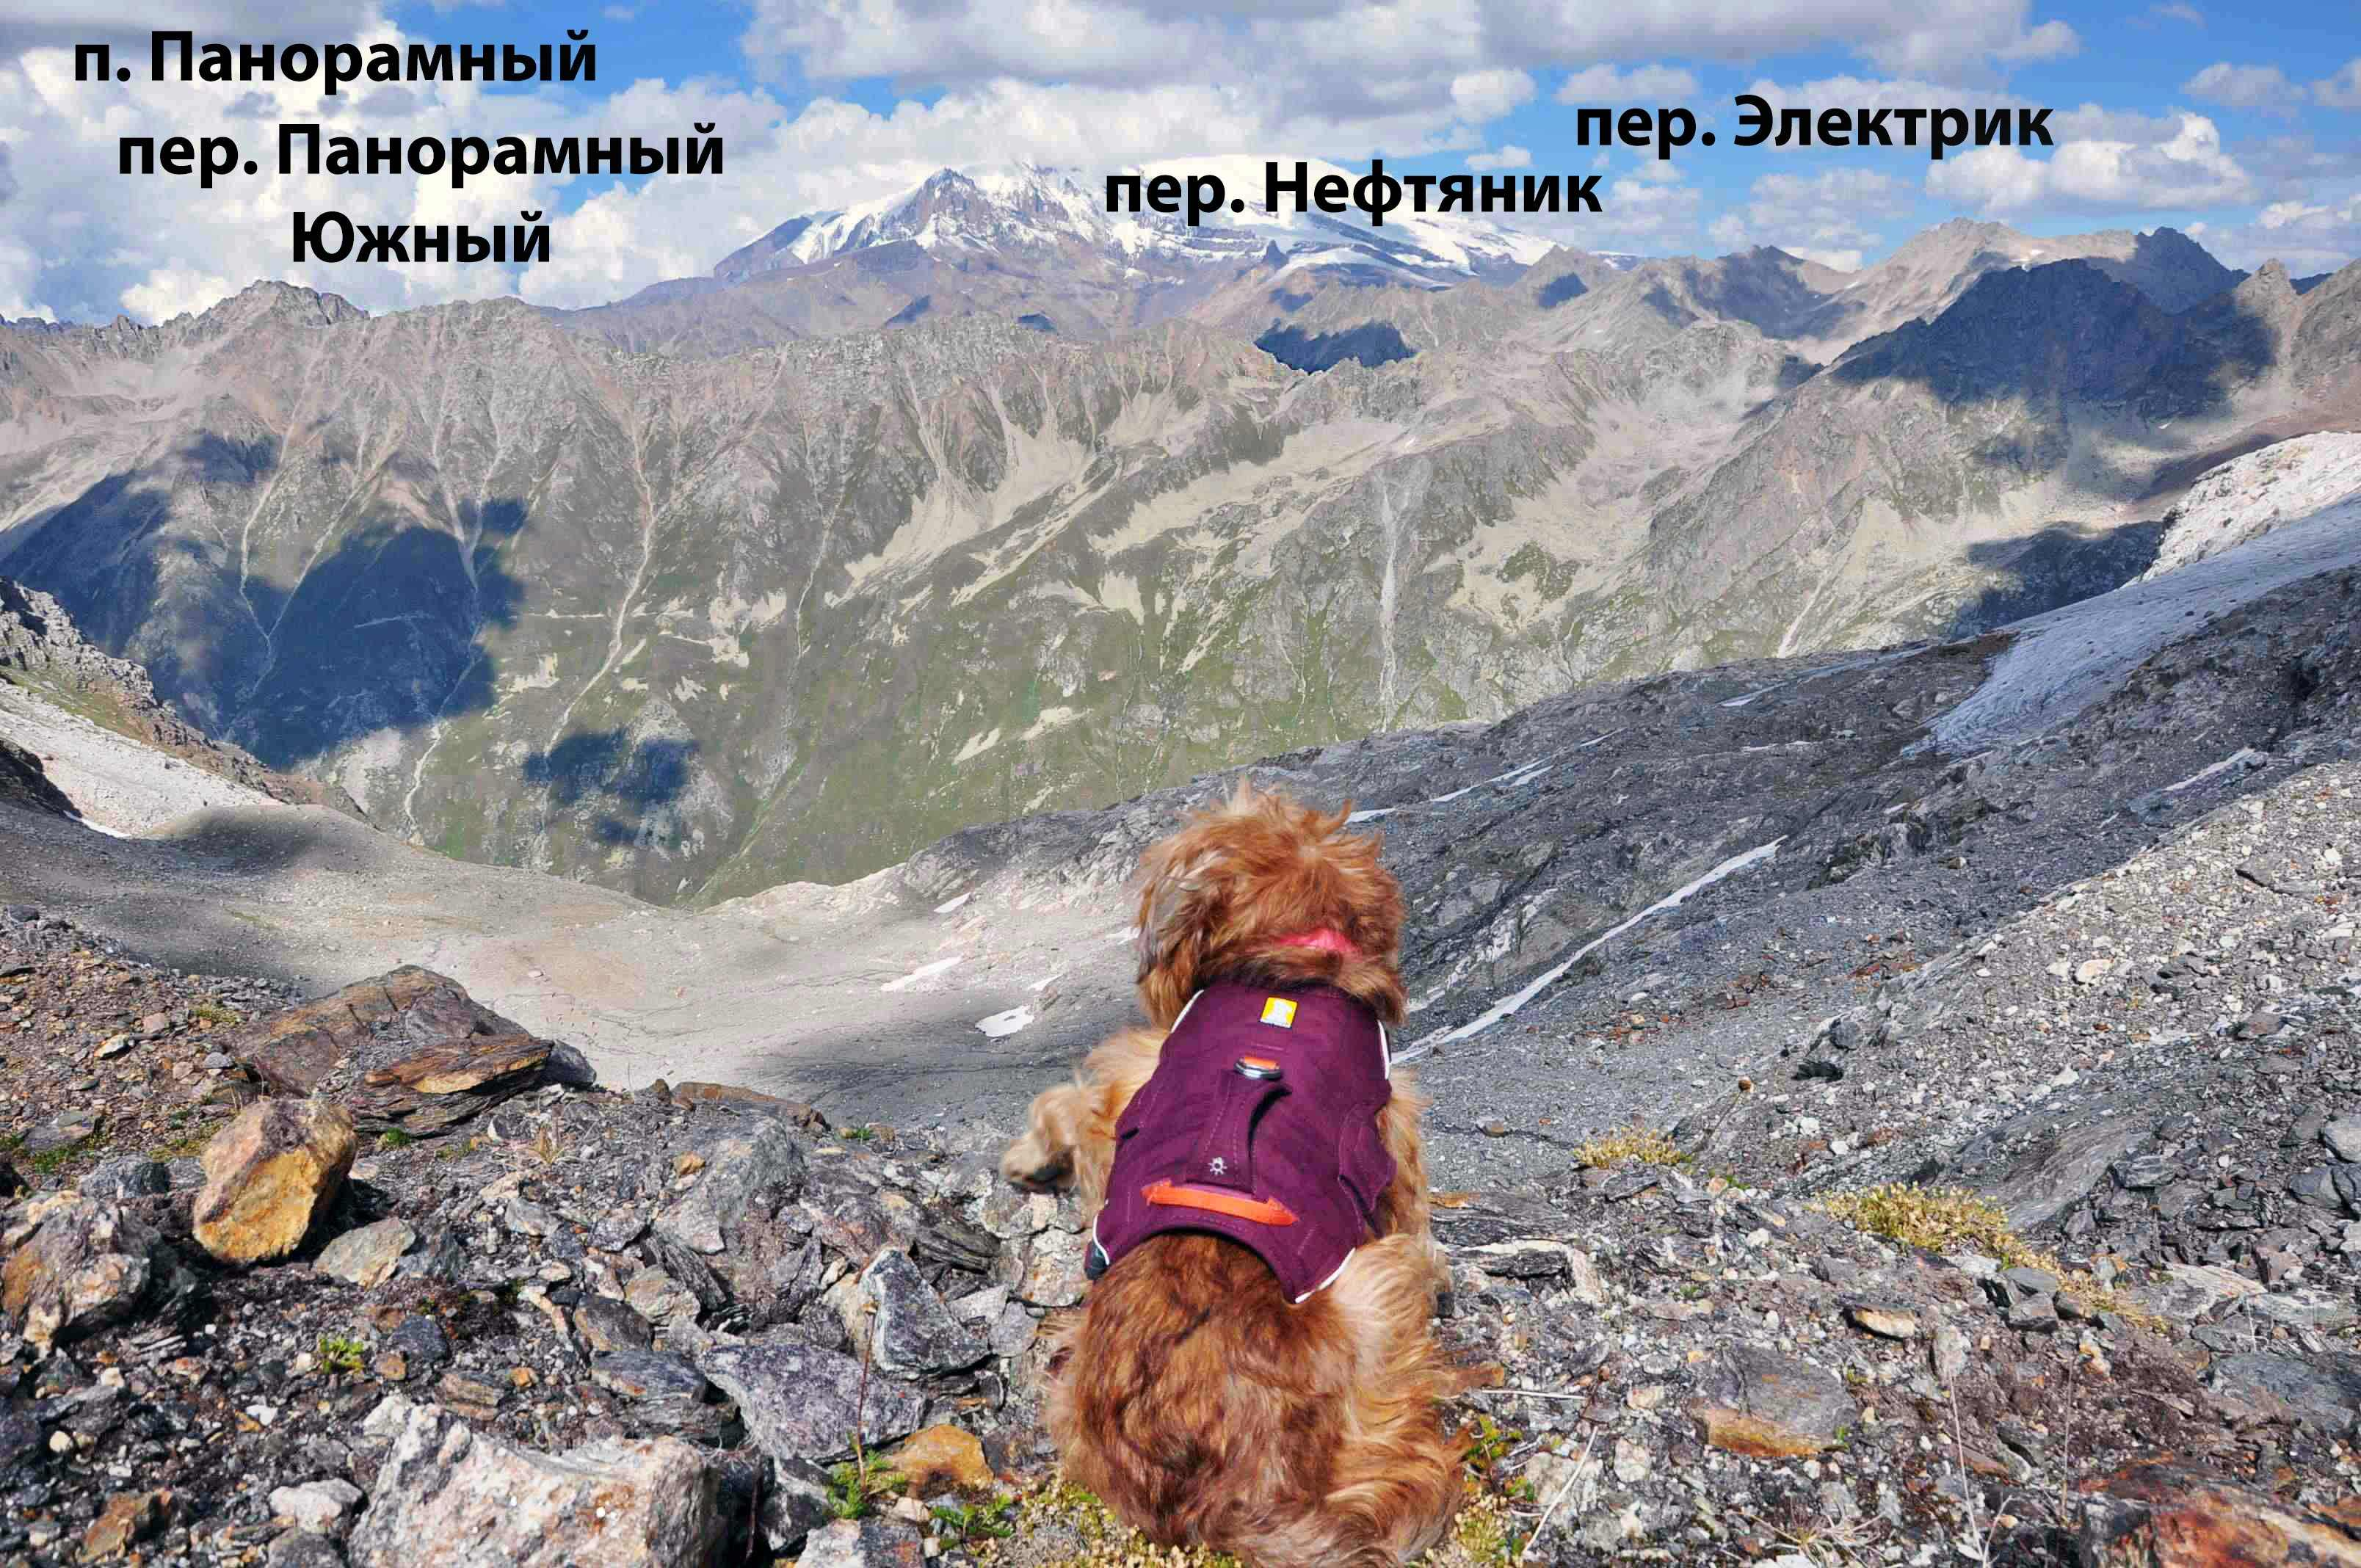
\includegraphics[width=0.7\linewidth]{../pics/DSC_0385 2.jpg}
	\caption{Вид с перевала в д.р. Танышхан}
	\label{fig:DSC_0385 2}
\end{figure} 


\textbf{Задача три:} спуститься в низ, в д.р. Танышхан. Здесь начинается очень интересная и поучительная история.
\begin{figure}[h!]
	\centering
	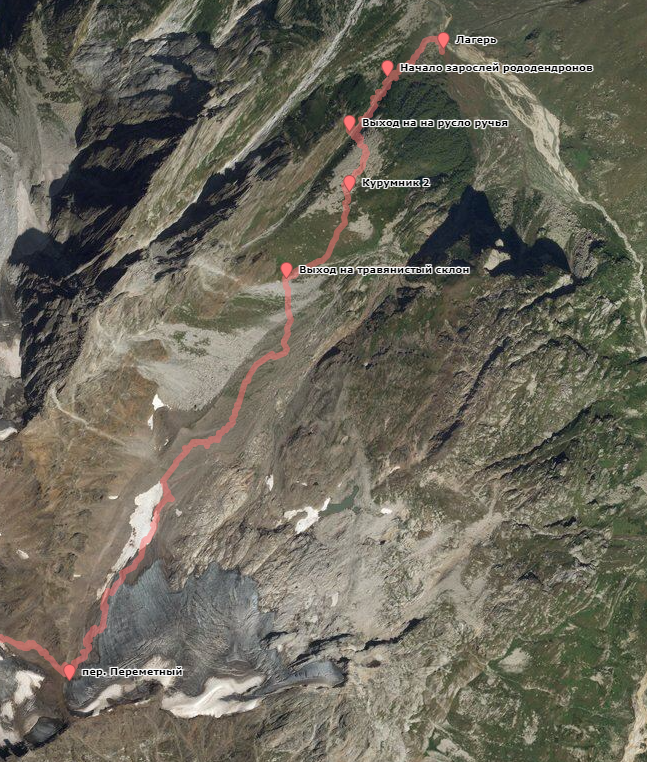
\includegraphics[width=0.7\linewidth]{../pics/perem_down.png}
	\caption{Спуск с перевала Перемётный}
	\label{perem_down}
\end{figure} 
Выдвинулись в 15:38. Вниз сначала шли по сыпухе забирая влево, усердно считали моренные валы чтобы не ошибиться и не угодить в березняк. По пути старались расставлять турики, но время подгоняло, в маршруте мы были не  уверены и на полпути мы это дело забросили.  Потом начался травянистый склон, альпеншток альпеншточил на все 100. После спуска на 130 м выбрались на курумник, на котором не обошлось без легкого кровопролития. К сумеркам снова вышли на травянистый склон. Русло пересохшего ручья (N 43.25779\degree E 42.27107\degree), засыпанного крупными камнями, предоставило удобный вариант до спуска. К моменту, когда мы добрались до зарослей рододендронов, уже порядком стемнело (19:05), дальше по лощине шли с фонарикам. 

В 20:00 вышли на отличную стоянку на берегу реки Танышхан (N 43.26002, E 42.27489). Поужинали и легли спать. С задачей три справились! 

\subparagraph{Описание от шефа} 

Спуск с перевала начали в 15:38. Согласно отчёту Анучиной \cite{Anuchina2019}, встать на стоянку можно было либо где-то в районе истока ручья, спустившись на 300 м ниже, либо уже в д/р Танышхан, сбросив полностью 900 м. Предполагалось, что практически наверняка реализуется первый, 300-метровый вариант. 

Первые 70 м спуска представляли из себя крутой осыпной склон, с живой осыпью среднего и крупного размера. Спускались по правому <<углу>> перевала, образованного собственно хребтом \textcolor{teal}{(каким?)} и отходящим от него гребнем. Шли плотной группой, зигзагом, с подстраховкой альпенштоком.  

Следующим этапом вышли на гребень моренного вала. Качество рельефа непосредственно на гребне не удовлетворило, поэтому моренный вал траверсировали по его правому борту, по серой вязкой осыпи, избегая полностью спускаться вниз --- чтобы не угодить под кромку снежника, который лежал с правой стороны от вала. \textcolor{teal}{(Время!)} 

После спуска с моренного вала шёл отличный пологий участок с постоянным уклоном и комфортным в плане перемещения рельефом, вплоть до выхода к истоку ручья \textcolor{teal}{(какого?)} и далее к краю  ступени. Эта ступень может рассматриваться как ближайшее к перевалу пригодное место для стоянки. Однако мы продолжили движение \textcolor{teal}{(А поч-чему?)} и, пересёкши \textcolor{textcolor}{(Аыаыаы!)} ручей, стали продвигаться влево, огибая траверсом первый <<зелёный бугор>>: участок склона, который с этого ракурса перекрывает вид на дальнейший маршрут спуска. \textcolor{teal}{(Время!)} 



Чо ещё добавить: 
\begin{enumerate} 
	\item Первые 70 м — крутой спуск по кулуарчику в правом углу; 
	\item Потом — спуск по вязкому серому конгломерату по правому борту моренного вала (не понизу, чтобі не угодить под снежничек); 
	\item По этому же моренному выносу — быстрый и лёгкий выход на первую сверху ступень. Оттуда открывается вид на реку, вдоль по которой нам нинада; 
	\item Пересекаем реку справа налево и начинаем подниматься на зелёный бугор (покрытый альпийским лугом). Огибаем бугор сраверсом. Над бугром высятся скалы, но это ещё не наш хребет; 
	\item  За первым зелёным бугром есть ещё один, сильно более крутым травяным склоном. Там имел место человеческий траверс\texttrademark
	\item Прошли Анучинское м.н. примерно в 17:20
	\item Начало злобной морені: 18:20. Поцелуй с курумом: 18:46, начало спуска по лощине: 19:26
\end{enumerate}

\begin{figure}[h!]
	\centering
	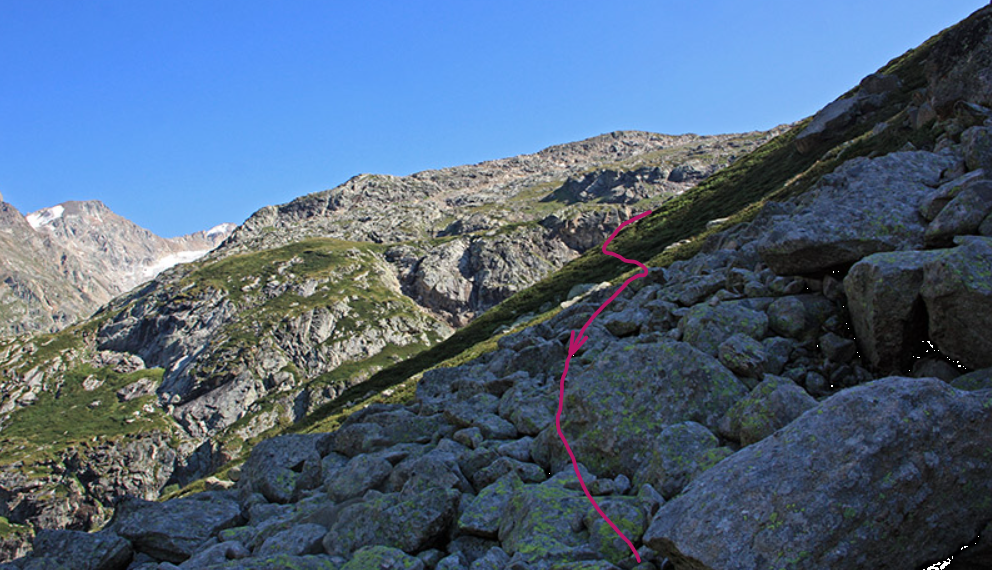
\includegraphics[width=0.7\linewidth]{../pics/peremkurum.png}
	\caption{Движение по курумнику. Фото Анучиной Светланы}
	\label{perem_down}
\end{figure} 


\begin{table}[h!]
	\centering
	\begin{tabular}{|c|c|c|c|c|c|} 
		\hline 
		Этап & ЧХВ \\ 	
		\hline 
		Подъём от места ночевки до языка ледника  & 02:41 \\
		Подъём от языка ледника до седловины  & 00:40 \\
		Спуск с седловины перевала Переметный до лощины & 02:41\\ 
		Спуск по лощине до д.р. Чиринкол & 01:23\\ 
		Спуск с места ночёвки до слияния рек Чиринкол и Кубань & 04:10 \\
		
		\hline
		\textsc{Полное время подъёма на перевал  }& 03:21\\
		\textsc{Полное время спуска с перевала }& 08:14 \\
		\textsc{Полное время прохождения перевала }& 11:35 \\
		\hline
	\end{tabular}
	\caption{Расклад времени, пер. Перемётный}
\end{table}

\paragraph{Выводы и рекомендации:} ок

\clearpage